\documentclass[11pt]{article}

    \usepackage[breakable]{tcolorbox}
    \usepackage{parskip} % Stop auto-indenting (to mimic markdown behaviour)
    
    \usepackage{iftex}
    \ifPDFTeX
    	\usepackage[T1]{fontenc}
    	\usepackage{mathpazo}
    \else
    	\usepackage{fontspec}
    \fi

    % Basic figure setup, for now with no caption control since it's done
    % automatically by Pandoc (which extracts ![](path) syntax from Markdown).
    \usepackage{graphicx}
    % Maintain compatibility with old templates. Remove in nbconvert 6.0
    \let\Oldincludegraphics\includegraphics
    % Ensure that by default, figures have no caption (until we provide a
    % proper Figure object with a Caption API and a way to capture that
    % in the conversion process - todo).
    \usepackage{caption}
    \DeclareCaptionFormat{nocaption}{}
    \captionsetup{format=nocaption,aboveskip=0pt,belowskip=0pt}

    \usepackage{float}
    \floatplacement{figure}{H} % forces figures to be placed at the correct location
    \usepackage{xcolor} % Allow colors to be defined
    \usepackage{enumerate} % Needed for markdown enumerations to work
    \usepackage{geometry} % Used to adjust the document margins
    \usepackage{amsmath} % Equations
    \usepackage{amssymb} % Equations
    \usepackage{textcomp} % defines textquotesingle
    % Hack from http://tex.stackexchange.com/a/47451/13684:
    \AtBeginDocument{%
        \def\PYZsq{\textquotesingle}% Upright quotes in Pygmentized code
    }
    \usepackage{upquote} % Upright quotes for verbatim code
    \usepackage{eurosym} % defines \euro
    \usepackage[mathletters]{ucs} % Extended unicode (utf-8) support
    \usepackage{fancyvrb} % verbatim replacement that allows latex
    \usepackage{grffile} % extends the file name processing of package graphics 
                         % to support a larger range
    \makeatletter % fix for old versions of grffile with XeLaTeX
    \@ifpackagelater{grffile}{2019/11/01}
    {
      % Do nothing on new versions
    }
    {
      \def\Gread@@xetex#1{%
        \IfFileExists{"\Gin@base".bb}%
        {\Gread@eps{\Gin@base.bb}}%
        {\Gread@@xetex@aux#1}%
      }
    }
    \makeatother
    \usepackage[Export]{adjustbox} % Used to constrain images to a maximum size
    \adjustboxset{max size={0.9\linewidth}{0.9\paperheight}}

    % The hyperref package gives us a pdf with properly built
    % internal navigation ('pdf bookmarks' for the table of contents,
    % internal cross-reference links, web links for URLs, etc.)
    \usepackage{hyperref}
    % The default LaTeX title has an obnoxious amount of whitespace. By default,
    % titling removes some of it. It also provides customization options.
    \usepackage{titling}
    \usepackage{longtable} % longtable support required by pandoc >1.10
    \usepackage{booktabs}  % table support for pandoc > 1.12.2
    \usepackage[inline]{enumitem} % IRkernel/repr support (it uses the enumerate* environment)
    \usepackage[normalem]{ulem} % ulem is needed to support strikethroughs (\sout)
                                % normalem makes italics be italics, not underlines
    \usepackage{mathrsfs}
    

    
    % Colors for the hyperref package
    \definecolor{urlcolor}{rgb}{0,.145,.698}
    \definecolor{linkcolor}{rgb}{.71,0.21,0.01}
    \definecolor{citecolor}{rgb}{.12,.54,.11}

    % ANSI colors
    \definecolor{ansi-black}{HTML}{3E424D}
    \definecolor{ansi-black-intense}{HTML}{282C36}
    \definecolor{ansi-red}{HTML}{E75C58}
    \definecolor{ansi-red-intense}{HTML}{B22B31}
    \definecolor{ansi-green}{HTML}{00A250}
    \definecolor{ansi-green-intense}{HTML}{007427}
    \definecolor{ansi-yellow}{HTML}{DDB62B}
    \definecolor{ansi-yellow-intense}{HTML}{B27D12}
    \definecolor{ansi-blue}{HTML}{208FFB}
    \definecolor{ansi-blue-intense}{HTML}{0065CA}
    \definecolor{ansi-magenta}{HTML}{D160C4}
    \definecolor{ansi-magenta-intense}{HTML}{A03196}
    \definecolor{ansi-cyan}{HTML}{60C6C8}
    \definecolor{ansi-cyan-intense}{HTML}{258F8F}
    \definecolor{ansi-white}{HTML}{C5C1B4}
    \definecolor{ansi-white-intense}{HTML}{A1A6B2}
    \definecolor{ansi-default-inverse-fg}{HTML}{FFFFFF}
    \definecolor{ansi-default-inverse-bg}{HTML}{000000}

    % common color for the border for error outputs.
    \definecolor{outerrorbackground}{HTML}{FFDFDF}

    % commands and environments needed by pandoc snippets
    % extracted from the output of `pandoc -s`
    \providecommand{\tightlist}{%
      \setlength{\itemsep}{0pt}\setlength{\parskip}{0pt}}
    \DefineVerbatimEnvironment{Highlighting}{Verbatim}{commandchars=\\\{\}}
    % Add ',fontsize=\small' for more characters per line
    \newenvironment{Shaded}{}{}
    \newcommand{\KeywordTok}[1]{\textcolor[rgb]{0.00,0.44,0.13}{\textbf{{#1}}}}
    \newcommand{\DataTypeTok}[1]{\textcolor[rgb]{0.56,0.13,0.00}{{#1}}}
    \newcommand{\DecValTok}[1]{\textcolor[rgb]{0.25,0.63,0.44}{{#1}}}
    \newcommand{\BaseNTok}[1]{\textcolor[rgb]{0.25,0.63,0.44}{{#1}}}
    \newcommand{\FloatTok}[1]{\textcolor[rgb]{0.25,0.63,0.44}{{#1}}}
    \newcommand{\CharTok}[1]{\textcolor[rgb]{0.25,0.44,0.63}{{#1}}}
    \newcommand{\StringTok}[1]{\textcolor[rgb]{0.25,0.44,0.63}{{#1}}}
    \newcommand{\CommentTok}[1]{\textcolor[rgb]{0.38,0.63,0.69}{\textit{{#1}}}}
    \newcommand{\OtherTok}[1]{\textcolor[rgb]{0.00,0.44,0.13}{{#1}}}
    \newcommand{\AlertTok}[1]{\textcolor[rgb]{1.00,0.00,0.00}{\textbf{{#1}}}}
    \newcommand{\FunctionTok}[1]{\textcolor[rgb]{0.02,0.16,0.49}{{#1}}}
    \newcommand{\RegionMarkerTok}[1]{{#1}}
    \newcommand{\ErrorTok}[1]{\textcolor[rgb]{1.00,0.00,0.00}{\textbf{{#1}}}}
    \newcommand{\NormalTok}[1]{{#1}}
    
    % Additional commands for more recent versions of Pandoc
    \newcommand{\ConstantTok}[1]{\textcolor[rgb]{0.53,0.00,0.00}{{#1}}}
    \newcommand{\SpecialCharTok}[1]{\textcolor[rgb]{0.25,0.44,0.63}{{#1}}}
    \newcommand{\VerbatimStringTok}[1]{\textcolor[rgb]{0.25,0.44,0.63}{{#1}}}
    \newcommand{\SpecialStringTok}[1]{\textcolor[rgb]{0.73,0.40,0.53}{{#1}}}
    \newcommand{\ImportTok}[1]{{#1}}
    \newcommand{\DocumentationTok}[1]{\textcolor[rgb]{0.73,0.13,0.13}{\textit{{#1}}}}
    \newcommand{\AnnotationTok}[1]{\textcolor[rgb]{0.38,0.63,0.69}{\textbf{\textit{{#1}}}}}
    \newcommand{\CommentVarTok}[1]{\textcolor[rgb]{0.38,0.63,0.69}{\textbf{\textit{{#1}}}}}
    \newcommand{\VariableTok}[1]{\textcolor[rgb]{0.10,0.09,0.49}{{#1}}}
    \newcommand{\ControlFlowTok}[1]{\textcolor[rgb]{0.00,0.44,0.13}{\textbf{{#1}}}}
    \newcommand{\OperatorTok}[1]{\textcolor[rgb]{0.40,0.40,0.40}{{#1}}}
    \newcommand{\BuiltInTok}[1]{{#1}}
    \newcommand{\ExtensionTok}[1]{{#1}}
    \newcommand{\PreprocessorTok}[1]{\textcolor[rgb]{0.74,0.48,0.00}{{#1}}}
    \newcommand{\AttributeTok}[1]{\textcolor[rgb]{0.49,0.56,0.16}{{#1}}}
    \newcommand{\InformationTok}[1]{\textcolor[rgb]{0.38,0.63,0.69}{\textbf{\textit{{#1}}}}}
    \newcommand{\WarningTok}[1]{\textcolor[rgb]{0.38,0.63,0.69}{\textbf{\textit{{#1}}}}}
    
    
    % Define a nice break command that doesn't care if a line doesn't already
    % exist.
    \def\br{\hspace*{\fill} \\* }
    % Math Jax compatibility definitions
    \def\gt{>}
    \def\lt{<}
    \let\Oldtex\TeX
    \let\Oldlatex\LaTeX
    \renewcommand{\TeX}{\textrm{\Oldtex}}
    \renewcommand{\LaTeX}{\textrm{\Oldlatex}}
    % Document parameters
    % Document title
    \title{chapter-4-2}
    
    
    
    
    
% Pygments definitions
\makeatletter
\def\PY@reset{\let\PY@it=\relax \let\PY@bf=\relax%
    \let\PY@ul=\relax \let\PY@tc=\relax%
    \let\PY@bc=\relax \let\PY@ff=\relax}
\def\PY@tok#1{\csname PY@tok@#1\endcsname}
\def\PY@toks#1+{\ifx\relax#1\empty\else%
    \PY@tok{#1}\expandafter\PY@toks\fi}
\def\PY@do#1{\PY@bc{\PY@tc{\PY@ul{%
    \PY@it{\PY@bf{\PY@ff{#1}}}}}}}
\def\PY#1#2{\PY@reset\PY@toks#1+\relax+\PY@do{#2}}

\@namedef{PY@tok@w}{\def\PY@tc##1{\textcolor[rgb]{0.73,0.73,0.73}{##1}}}
\@namedef{PY@tok@c}{\let\PY@it=\textit\def\PY@tc##1{\textcolor[rgb]{0.25,0.50,0.50}{##1}}}
\@namedef{PY@tok@cp}{\def\PY@tc##1{\textcolor[rgb]{0.74,0.48,0.00}{##1}}}
\@namedef{PY@tok@k}{\let\PY@bf=\textbf\def\PY@tc##1{\textcolor[rgb]{0.00,0.50,0.00}{##1}}}
\@namedef{PY@tok@kp}{\def\PY@tc##1{\textcolor[rgb]{0.00,0.50,0.00}{##1}}}
\@namedef{PY@tok@kt}{\def\PY@tc##1{\textcolor[rgb]{0.69,0.00,0.25}{##1}}}
\@namedef{PY@tok@o}{\def\PY@tc##1{\textcolor[rgb]{0.40,0.40,0.40}{##1}}}
\@namedef{PY@tok@ow}{\let\PY@bf=\textbf\def\PY@tc##1{\textcolor[rgb]{0.67,0.13,1.00}{##1}}}
\@namedef{PY@tok@nb}{\def\PY@tc##1{\textcolor[rgb]{0.00,0.50,0.00}{##1}}}
\@namedef{PY@tok@nf}{\def\PY@tc##1{\textcolor[rgb]{0.00,0.00,1.00}{##1}}}
\@namedef{PY@tok@nc}{\let\PY@bf=\textbf\def\PY@tc##1{\textcolor[rgb]{0.00,0.00,1.00}{##1}}}
\@namedef{PY@tok@nn}{\let\PY@bf=\textbf\def\PY@tc##1{\textcolor[rgb]{0.00,0.00,1.00}{##1}}}
\@namedef{PY@tok@ne}{\let\PY@bf=\textbf\def\PY@tc##1{\textcolor[rgb]{0.82,0.25,0.23}{##1}}}
\@namedef{PY@tok@nv}{\def\PY@tc##1{\textcolor[rgb]{0.10,0.09,0.49}{##1}}}
\@namedef{PY@tok@no}{\def\PY@tc##1{\textcolor[rgb]{0.53,0.00,0.00}{##1}}}
\@namedef{PY@tok@nl}{\def\PY@tc##1{\textcolor[rgb]{0.63,0.63,0.00}{##1}}}
\@namedef{PY@tok@ni}{\let\PY@bf=\textbf\def\PY@tc##1{\textcolor[rgb]{0.60,0.60,0.60}{##1}}}
\@namedef{PY@tok@na}{\def\PY@tc##1{\textcolor[rgb]{0.49,0.56,0.16}{##1}}}
\@namedef{PY@tok@nt}{\let\PY@bf=\textbf\def\PY@tc##1{\textcolor[rgb]{0.00,0.50,0.00}{##1}}}
\@namedef{PY@tok@nd}{\def\PY@tc##1{\textcolor[rgb]{0.67,0.13,1.00}{##1}}}
\@namedef{PY@tok@s}{\def\PY@tc##1{\textcolor[rgb]{0.73,0.13,0.13}{##1}}}
\@namedef{PY@tok@sd}{\let\PY@it=\textit\def\PY@tc##1{\textcolor[rgb]{0.73,0.13,0.13}{##1}}}
\@namedef{PY@tok@si}{\let\PY@bf=\textbf\def\PY@tc##1{\textcolor[rgb]{0.73,0.40,0.53}{##1}}}
\@namedef{PY@tok@se}{\let\PY@bf=\textbf\def\PY@tc##1{\textcolor[rgb]{0.73,0.40,0.13}{##1}}}
\@namedef{PY@tok@sr}{\def\PY@tc##1{\textcolor[rgb]{0.73,0.40,0.53}{##1}}}
\@namedef{PY@tok@ss}{\def\PY@tc##1{\textcolor[rgb]{0.10,0.09,0.49}{##1}}}
\@namedef{PY@tok@sx}{\def\PY@tc##1{\textcolor[rgb]{0.00,0.50,0.00}{##1}}}
\@namedef{PY@tok@m}{\def\PY@tc##1{\textcolor[rgb]{0.40,0.40,0.40}{##1}}}
\@namedef{PY@tok@gh}{\let\PY@bf=\textbf\def\PY@tc##1{\textcolor[rgb]{0.00,0.00,0.50}{##1}}}
\@namedef{PY@tok@gu}{\let\PY@bf=\textbf\def\PY@tc##1{\textcolor[rgb]{0.50,0.00,0.50}{##1}}}
\@namedef{PY@tok@gd}{\def\PY@tc##1{\textcolor[rgb]{0.63,0.00,0.00}{##1}}}
\@namedef{PY@tok@gi}{\def\PY@tc##1{\textcolor[rgb]{0.00,0.63,0.00}{##1}}}
\@namedef{PY@tok@gr}{\def\PY@tc##1{\textcolor[rgb]{1.00,0.00,0.00}{##1}}}
\@namedef{PY@tok@ge}{\let\PY@it=\textit}
\@namedef{PY@tok@gs}{\let\PY@bf=\textbf}
\@namedef{PY@tok@gp}{\let\PY@bf=\textbf\def\PY@tc##1{\textcolor[rgb]{0.00,0.00,0.50}{##1}}}
\@namedef{PY@tok@go}{\def\PY@tc##1{\textcolor[rgb]{0.53,0.53,0.53}{##1}}}
\@namedef{PY@tok@gt}{\def\PY@tc##1{\textcolor[rgb]{0.00,0.27,0.87}{##1}}}
\@namedef{PY@tok@err}{\def\PY@bc##1{{\setlength{\fboxsep}{\string -\fboxrule}\fcolorbox[rgb]{1.00,0.00,0.00}{1,1,1}{\strut ##1}}}}
\@namedef{PY@tok@kc}{\let\PY@bf=\textbf\def\PY@tc##1{\textcolor[rgb]{0.00,0.50,0.00}{##1}}}
\@namedef{PY@tok@kd}{\let\PY@bf=\textbf\def\PY@tc##1{\textcolor[rgb]{0.00,0.50,0.00}{##1}}}
\@namedef{PY@tok@kn}{\let\PY@bf=\textbf\def\PY@tc##1{\textcolor[rgb]{0.00,0.50,0.00}{##1}}}
\@namedef{PY@tok@kr}{\let\PY@bf=\textbf\def\PY@tc##1{\textcolor[rgb]{0.00,0.50,0.00}{##1}}}
\@namedef{PY@tok@bp}{\def\PY@tc##1{\textcolor[rgb]{0.00,0.50,0.00}{##1}}}
\@namedef{PY@tok@fm}{\def\PY@tc##1{\textcolor[rgb]{0.00,0.00,1.00}{##1}}}
\@namedef{PY@tok@vc}{\def\PY@tc##1{\textcolor[rgb]{0.10,0.09,0.49}{##1}}}
\@namedef{PY@tok@vg}{\def\PY@tc##1{\textcolor[rgb]{0.10,0.09,0.49}{##1}}}
\@namedef{PY@tok@vi}{\def\PY@tc##1{\textcolor[rgb]{0.10,0.09,0.49}{##1}}}
\@namedef{PY@tok@vm}{\def\PY@tc##1{\textcolor[rgb]{0.10,0.09,0.49}{##1}}}
\@namedef{PY@tok@sa}{\def\PY@tc##1{\textcolor[rgb]{0.73,0.13,0.13}{##1}}}
\@namedef{PY@tok@sb}{\def\PY@tc##1{\textcolor[rgb]{0.73,0.13,0.13}{##1}}}
\@namedef{PY@tok@sc}{\def\PY@tc##1{\textcolor[rgb]{0.73,0.13,0.13}{##1}}}
\@namedef{PY@tok@dl}{\def\PY@tc##1{\textcolor[rgb]{0.73,0.13,0.13}{##1}}}
\@namedef{PY@tok@s2}{\def\PY@tc##1{\textcolor[rgb]{0.73,0.13,0.13}{##1}}}
\@namedef{PY@tok@sh}{\def\PY@tc##1{\textcolor[rgb]{0.73,0.13,0.13}{##1}}}
\@namedef{PY@tok@s1}{\def\PY@tc##1{\textcolor[rgb]{0.73,0.13,0.13}{##1}}}
\@namedef{PY@tok@mb}{\def\PY@tc##1{\textcolor[rgb]{0.40,0.40,0.40}{##1}}}
\@namedef{PY@tok@mf}{\def\PY@tc##1{\textcolor[rgb]{0.40,0.40,0.40}{##1}}}
\@namedef{PY@tok@mh}{\def\PY@tc##1{\textcolor[rgb]{0.40,0.40,0.40}{##1}}}
\@namedef{PY@tok@mi}{\def\PY@tc##1{\textcolor[rgb]{0.40,0.40,0.40}{##1}}}
\@namedef{PY@tok@il}{\def\PY@tc##1{\textcolor[rgb]{0.40,0.40,0.40}{##1}}}
\@namedef{PY@tok@mo}{\def\PY@tc##1{\textcolor[rgb]{0.40,0.40,0.40}{##1}}}
\@namedef{PY@tok@ch}{\let\PY@it=\textit\def\PY@tc##1{\textcolor[rgb]{0.25,0.50,0.50}{##1}}}
\@namedef{PY@tok@cm}{\let\PY@it=\textit\def\PY@tc##1{\textcolor[rgb]{0.25,0.50,0.50}{##1}}}
\@namedef{PY@tok@cpf}{\let\PY@it=\textit\def\PY@tc##1{\textcolor[rgb]{0.25,0.50,0.50}{##1}}}
\@namedef{PY@tok@c1}{\let\PY@it=\textit\def\PY@tc##1{\textcolor[rgb]{0.25,0.50,0.50}{##1}}}
\@namedef{PY@tok@cs}{\let\PY@it=\textit\def\PY@tc##1{\textcolor[rgb]{0.25,0.50,0.50}{##1}}}

\def\PYZbs{\char`\\}
\def\PYZus{\char`\_}
\def\PYZob{\char`\{}
\def\PYZcb{\char`\}}
\def\PYZca{\char`\^}
\def\PYZam{\char`\&}
\def\PYZlt{\char`\<}
\def\PYZgt{\char`\>}
\def\PYZsh{\char`\#}
\def\PYZpc{\char`\%}
\def\PYZdl{\char`\$}
\def\PYZhy{\char`\-}
\def\PYZsq{\char`\'}
\def\PYZdq{\char`\"}
\def\PYZti{\char`\~}
% for compatibility with earlier versions
\def\PYZat{@}
\def\PYZlb{[}
\def\PYZrb{]}
\makeatother


    % For linebreaks inside Verbatim environment from package fancyvrb. 
    \makeatletter
        \newbox\Wrappedcontinuationbox 
        \newbox\Wrappedvisiblespacebox 
        \newcommand*\Wrappedvisiblespace {\textcolor{red}{\textvisiblespace}} 
        \newcommand*\Wrappedcontinuationsymbol {\textcolor{red}{\llap{\tiny$\m@th\hookrightarrow$}}} 
        \newcommand*\Wrappedcontinuationindent {3ex } 
        \newcommand*\Wrappedafterbreak {\kern\Wrappedcontinuationindent\copy\Wrappedcontinuationbox} 
        % Take advantage of the already applied Pygments mark-up to insert 
        % potential linebreaks for TeX processing. 
        %        {, <, #, %, $, ' and ": go to next line. 
        %        _, }, ^, &, >, - and ~: stay at end of broken line. 
        % Use of \textquotesingle for straight quote. 
        \newcommand*\Wrappedbreaksatspecials {% 
            \def\PYGZus{\discretionary{\char`\_}{\Wrappedafterbreak}{\char`\_}}% 
            \def\PYGZob{\discretionary{}{\Wrappedafterbreak\char`\{}{\char`\{}}% 
            \def\PYGZcb{\discretionary{\char`\}}{\Wrappedafterbreak}{\char`\}}}% 
            \def\PYGZca{\discretionary{\char`\^}{\Wrappedafterbreak}{\char`\^}}% 
            \def\PYGZam{\discretionary{\char`\&}{\Wrappedafterbreak}{\char`\&}}% 
            \def\PYGZlt{\discretionary{}{\Wrappedafterbreak\char`\<}{\char`\<}}% 
            \def\PYGZgt{\discretionary{\char`\>}{\Wrappedafterbreak}{\char`\>}}% 
            \def\PYGZsh{\discretionary{}{\Wrappedafterbreak\char`\#}{\char`\#}}% 
            \def\PYGZpc{\discretionary{}{\Wrappedafterbreak\char`\%}{\char`\%}}% 
            \def\PYGZdl{\discretionary{}{\Wrappedafterbreak\char`\$}{\char`\$}}% 
            \def\PYGZhy{\discretionary{\char`\-}{\Wrappedafterbreak}{\char`\-}}% 
            \def\PYGZsq{\discretionary{}{\Wrappedafterbreak\textquotesingle}{\textquotesingle}}% 
            \def\PYGZdq{\discretionary{}{\Wrappedafterbreak\char`\"}{\char`\"}}% 
            \def\PYGZti{\discretionary{\char`\~}{\Wrappedafterbreak}{\char`\~}}% 
        } 
        % Some characters . , ; ? ! / are not pygmentized. 
        % This macro makes them "active" and they will insert potential linebreaks 
        \newcommand*\Wrappedbreaksatpunct {% 
            \lccode`\~`\.\lowercase{\def~}{\discretionary{\hbox{\char`\.}}{\Wrappedafterbreak}{\hbox{\char`\.}}}% 
            \lccode`\~`\,\lowercase{\def~}{\discretionary{\hbox{\char`\,}}{\Wrappedafterbreak}{\hbox{\char`\,}}}% 
            \lccode`\~`\;\lowercase{\def~}{\discretionary{\hbox{\char`\;}}{\Wrappedafterbreak}{\hbox{\char`\;}}}% 
            \lccode`\~`\:\lowercase{\def~}{\discretionary{\hbox{\char`\:}}{\Wrappedafterbreak}{\hbox{\char`\:}}}% 
            \lccode`\~`\?\lowercase{\def~}{\discretionary{\hbox{\char`\?}}{\Wrappedafterbreak}{\hbox{\char`\?}}}% 
            \lccode`\~`\!\lowercase{\def~}{\discretionary{\hbox{\char`\!}}{\Wrappedafterbreak}{\hbox{\char`\!}}}% 
            \lccode`\~`\/\lowercase{\def~}{\discretionary{\hbox{\char`\/}}{\Wrappedafterbreak}{\hbox{\char`\/}}}% 
            \catcode`\.\active
            \catcode`\,\active 
            \catcode`\;\active
            \catcode`\:\active
            \catcode`\?\active
            \catcode`\!\active
            \catcode`\/\active 
            \lccode`\~`\~ 	
        }
    \makeatother

    \let\OriginalVerbatim=\Verbatim
    \makeatletter
    \renewcommand{\Verbatim}[1][1]{%
        %\parskip\z@skip
        \sbox\Wrappedcontinuationbox {\Wrappedcontinuationsymbol}%
        \sbox\Wrappedvisiblespacebox {\FV@SetupFont\Wrappedvisiblespace}%
        \def\FancyVerbFormatLine ##1{\hsize\linewidth
            \vtop{\raggedright\hyphenpenalty\z@\exhyphenpenalty\z@
                \doublehyphendemerits\z@\finalhyphendemerits\z@
                \strut ##1\strut}%
        }%
        % If the linebreak is at a space, the latter will be displayed as visible
        % space at end of first line, and a continuation symbol starts next line.
        % Stretch/shrink are however usually zero for typewriter font.
        \def\FV@Space {%
            \nobreak\hskip\z@ plus\fontdimen3\font minus\fontdimen4\font
            \discretionary{\copy\Wrappedvisiblespacebox}{\Wrappedafterbreak}
            {\kern\fontdimen2\font}%
        }%
        
        % Allow breaks at special characters using \PYG... macros.
        \Wrappedbreaksatspecials
        % Breaks at punctuation characters . , ; ? ! and / need catcode=\active 	
        \OriginalVerbatim[#1,codes*=\Wrappedbreaksatpunct]%
    }
    \makeatother

    % Exact colors from NB
    \definecolor{incolor}{HTML}{303F9F}
    \definecolor{outcolor}{HTML}{D84315}
    \definecolor{cellborder}{HTML}{CFCFCF}
    \definecolor{cellbackground}{HTML}{F7F7F7}
    
    % prompt
    \makeatletter
    \newcommand{\boxspacing}{\kern\kvtcb@left@rule\kern\kvtcb@boxsep}
    \makeatother
    \newcommand{\prompt}[4]{
        {\ttfamily\llap{{\color{#2}[#3]:\hspace{3pt}#4}}\vspace{-\baselineskip}}
    }
    

    
    % Prevent overflowing lines due to hard-to-break entities
    \sloppy 
    % Setup hyperref package
    \hypersetup{
      breaklinks=true,  % so long urls are correctly broken across lines
      colorlinks=true,
      urlcolor=urlcolor,
      linkcolor=linkcolor,
      citecolor=citecolor,
      }
    % Slightly bigger margins than the latex defaults
    
    \geometry{verbose,tmargin=1in,bmargin=1in,lmargin=1in,rmargin=1in}
    
    

\begin{document}
    
    \maketitle
    
    

    
    Run in Google Colab

    \textbf{TO BE DONE}

\begin{itemize}
\tightlist
\item
  Random Forest e ensamble methods
\end{itemize}

    \hypertarget{supervised-models-decision-trees}{%
\section{Supervised Models: Decision
Trees}\label{supervised-models-decision-trees}}

    \hypertarget{what-is-a-decision-tree}{%
\subsection{What is a decision tree?}\label{what-is-a-decision-tree}}

Decision trees can be used for regression (continuous real-valued
output, e.g.~predicting the price of a house) or classification
(categorical output, e.g.~predicting email spam vs.~no spam), but here
we will focus on classification. \textbf{A decision tree classifier is a
binary tree where predictions are made by traversing the tree from root
to leaf --- at each node, we go left if a feature is less than a
threshold, right otherwise. Finally, each leaf is associated with a
class, which is the output of the predictor}.

\hypertarget{why-decision-trees}{%
\subsubsection{Why Decision Trees?}\label{why-decision-trees}}

\begin{itemize}
\item
  Decision tress often mimic the human level thinking so its so simple
  to understand the data and make some good interpretations;
\item
  Decision trees actually make you see the logic for the data to
  interpret(not like black box algorithms like SVM,NN,etc..);
\item
  There is non requirement that the relationship between the target and
  the features be linear;
\item
  The tree automatically selects the best features to make the
  prediction;
\item
  A decision tree is less sensitive to outlying observations than a
  regression.
\end{itemize}

For example : if we are classifying bank loan application for a
customer, the decision tree may look like this Here we can see the logic
how it is making the decision.

    \begin{figure}
\centering
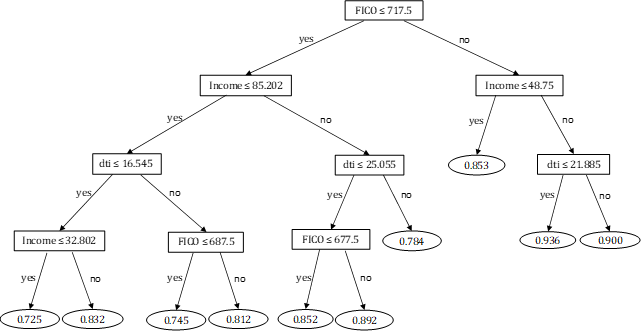
\includegraphics{./pic/chapter-4-2_pic_6.png}
\caption{chapter-4-2\_pic\_6-2.png}
\end{figure}

    It's simple and clear. So what is the decision tree?

    \hypertarget{building-a-decision-tree}{%
\subsection{Building a Decision Tree}\label{building-a-decision-tree}}

During model training on feature-target relationships, a tree is grown
from a \textbf{root} (parent) node (all data containing feature-target
relationships), which is then recursively split into child nodes (subset
of the entire data) in a binary fashion. Generally, each split is
performed on a single feature in the parent node. You will have
different kind of splitting depending on the nature of the feature:

\begin{itemize}
\tightlist
\item
  you can have a very simple decision tree in which the decision is a
  boolean condition (true, false) \ldots{}
\item
  \ldots{} or numeric data
\end{itemize}

In the last case we have to define a desired \textbf{threshold} value of
the feature. For instance, during each split of the parent node, we go
to left node (with the corresponding subset of data) if a feature is
less than the threshold, and right node otherwise. But how do we decide
on the split? The feature to put at the root node is the one with the
most \textbf{information gain}.

    \hypertarget{the-impurity-concept}{%
\subsubsection{The Impurity Concept}\label{the-impurity-concept}}

Decision trees use the concept of \textbf{impurity} to describe how
homogeneous or ``pure'' a node is. \textbf{A node is pure if all its
samples belong to the same class}, while \textbf{a node with many
samples from many different classes is called impure}. The difference
between the impurity of a node and that of the child nodes is called
\textbf{Information Gain}.

The goal of a decision tree is, at each layer, to try to split the data
into two (or more) groups, \textbf{so that data that fall into the same
group are most similar to each other (homogeneity), and groups are as
different as possible from each other (heterogeneity)}.

    In order to split the nodes at the most informative features, we need to
define an objective function that we want to optimize via the tree
learning algorithm. Here, our objective function is to maximize the
\textbf{IG} at each split, which we define as follows:

\begin{equation}
IG(D_p, f) = I(D_p) - \sum\limits_{j=1}^m \frac{N_j}{N_p} I(D_j)
\end{equation}

Here,

\begin{itemize}
\tightlist
\item
  \(f\) is the feature to perform the split;
\item
  \(𝐷_𝑝\) and \(𝐷_𝑗\) are the dataset of the parent and \(jth\) child
  node;
\item
  \(I\) is our impurity measure;
\item
  \(𝑁_𝑝\) is the total number of training examples at the parent node;
\item
  and \(𝑁_𝑗\) is the number of examples in the jth child node.
\end{itemize}

As we can see, the information gain is simply the difference between the
impurity of the parent node and the sum of the child node
impurities---the lower the impurities of the child nodes, the larger the
information gain. However, for simplicity and to reduce the
combinatorial search space, most libraries (including scikit-learn)
implement binary decision trees. This means that each parent node is
split into two child nodes, \(D_{left}\) and \(D_{right}\):

\begin{equation}
IG(D_p, f) = I(D_p) - \frac{N_{left}}{N_p}I(D_{left}) -
\frac{N_{right}}{N_p} I(D_{right})
\end{equation}

    \hypertarget{measures-of-information-gain}{%
\subsubsection{Measures of Information
Gain}\label{measures-of-information-gain}}

The three impurity measures or splitting criteria that are commonly used
in binary decision trees are \textbf{Entropy} \((𝐼_𝐻)\), \textbf{Gini
impurity} \((𝐼_𝐺)\) and the \textbf{Classification Error} \((𝐼_𝐸)\). In
the following we will focus only on the first two.

    \hypertarget{entropy}{%
\paragraph{Entropy}\label{entropy}}

One measure of information gain is based on \emph{entropy}.

Suppose that there are \(n\) possible outcomes and \(p_i\) is the
probability of outcome \(i\) with \(\sum\limits_{i=1}^n\, p_i=1\),
entropy can be defined as:
\[\text{Entropy}=-\sum\limits_{i=1}^n\, p_i \,\ln(p_i)\]

For example let's suppose some data for job application and we find that
the 20\% of them received an offer. Suppose further that 50\% of job
applicants have a relevant degree. If both those with a relevant degree
and those without a relevant degree had a 20\% chance of receiving a job
offer, there would be no information gain to knowing wheter an applicant
has a relevant degree. Suppose however that: - 30\% of those with a
relevant degree received a job offer - 10\% of those without a relevant
degree received a job offer

then there is clearly some information gain to knowing whether an
applicant has a relevant degree. Let's calculate the information gain
with entropy as a measure.

    \begin{tcolorbox}[breakable, size=fbox, boxrule=1pt, pad at break*=1mm,colback=cellbackground, colframe=cellborder]
\prompt{In}{incolor}{150}{\boxspacing}
\begin{Verbatim}[commandchars=\\\{\}]
\PY{k+kn}{import} \PY{n+nn}{math}

\PY{c+c1}{\PYZsh{} initial entropy, the only information we have is that 20\PYZpc{} of applicants find a job}
\PY{n}{p} \PY{o}{=} \PY{l+m+mf}{0.2}

\PY{n}{entropy\PYZus{}ini} \PY{o}{=} \PY{o}{\PYZhy{}}\PY{n}{p}\PY{o}{*}\PY{n}{math}\PY{o}{.}\PY{n}{log}\PY{p}{(}\PY{n}{p}\PY{p}{)} \PY{o}{\PYZhy{}} \PY{p}{(}\PY{l+m+mi}{1}\PY{o}{\PYZhy{}}\PY{n}{p}\PY{p}{)}\PY{o}{*}\PY{n}{math}\PY{o}{.}\PY{n}{log}\PY{p}{(}\PY{l+m+mi}{1}\PY{o}{\PYZhy{}}\PY{n}{p}\PY{p}{)}
\PY{n+nb}{print}\PY{p}{(}\PY{n}{entropy\PYZus{}ini}\PY{p}{)}
\end{Verbatim}
\end{tcolorbox}

    \begin{Verbatim}[commandchars=\\\{\}]
0.5004024235381879
    \end{Verbatim}

    If a candidate has a relevant degree this becomes

    \begin{tcolorbox}[breakable, size=fbox, boxrule=1pt, pad at break*=1mm,colback=cellbackground, colframe=cellborder]
\prompt{In}{incolor}{151}{\boxspacing}
\begin{Verbatim}[commandchars=\\\{\}]
\PY{n}{p} \PY{o}{=} \PY{l+m+mf}{0.3}

\PY{n}{entropy\PYZus{}1} \PY{o}{=} \PY{o}{\PYZhy{}}\PY{n}{p}\PY{o}{*}\PY{n}{math}\PY{o}{.}\PY{n}{log}\PY{p}{(}\PY{n}{p}\PY{p}{)} \PY{o}{\PYZhy{}} \PY{p}{(}\PY{l+m+mi}{1}\PY{o}{\PYZhy{}}\PY{n}{p}\PY{p}{)}\PY{o}{*}\PY{n}{math}\PY{o}{.}\PY{n}{log}\PY{p}{(}\PY{l+m+mi}{1}\PY{o}{\PYZhy{}}\PY{n}{p}\PY{p}{)}
\PY{n+nb}{print}\PY{p}{(}\PY{n}{entropy\PYZus{}1}\PY{p}{)}
\end{Verbatim}
\end{tcolorbox}

    \begin{Verbatim}[commandchars=\\\{\}]
0.6108643020548935
    \end{Verbatim}

    if a candidate does not have a relevant degree:

    \begin{tcolorbox}[breakable, size=fbox, boxrule=1pt, pad at break*=1mm,colback=cellbackground, colframe=cellborder]
\prompt{In}{incolor}{152}{\boxspacing}
\begin{Verbatim}[commandchars=\\\{\}]
\PY{n}{p} \PY{o}{=} \PY{l+m+mf}{0.1}

\PY{n}{entropy\PYZus{}2} \PY{o}{=} \PY{o}{\PYZhy{}}\PY{n}{p}\PY{o}{*}\PY{n}{math}\PY{o}{.}\PY{n}{log}\PY{p}{(}\PY{n}{p}\PY{p}{)} \PY{o}{\PYZhy{}} \PY{p}{(}\PY{l+m+mi}{1}\PY{o}{\PYZhy{}}\PY{n}{p}\PY{p}{)}\PY{o}{*}\PY{n}{math}\PY{o}{.}\PY{n}{log}\PY{p}{(}\PY{l+m+mi}{1}\PY{o}{\PYZhy{}}\PY{n}{p}\PY{p}{)}
\PY{n+nb}{print}\PY{p}{(}\PY{n}{entropy\PYZus{}2}\PY{p}{)}
\end{Verbatim}
\end{tcolorbox}

    \begin{Verbatim}[commandchars=\\\{\}]
0.3250829733914482
    \end{Verbatim}

    Because 50\% of candidates have a relevant degree, the expected value of
entropy after it is determined whether a candidate has a relevant degree
is

    \begin{tcolorbox}[breakable, size=fbox, boxrule=1pt, pad at break*=1mm,colback=cellbackground, colframe=cellborder]
\prompt{In}{incolor}{153}{\boxspacing}
\begin{Verbatim}[commandchars=\\\{\}]
\PY{n}{entropy\PYZus{}exp} \PY{o}{=} \PY{o}{.}\PY{l+m+mi}{5}\PY{o}{*}\PY{n}{entropy\PYZus{}1} \PY{o}{+} \PY{l+m+mf}{0.5}\PY{o}{*}\PY{n}{entropy\PYZus{}2}
\PY{n+nb}{print}\PY{p}{(}\PY{l+s+s1}{\PYZsq{}}\PY{l+s+s1}{Expected Entropy = }\PY{l+s+s1}{\PYZsq{}} \PY{o}{+} \PY{n+nb}{str}\PY{p}{(}\PY{n}{entropy\PYZus{}exp}\PY{p}{)} \PY{o}{+} \PY{l+s+s1}{\PYZsq{}}\PY{l+s+se}{\PYZbs{}n}\PY{l+s+s1}{\PYZsq{}}\PY{p}{)}
\PY{c+c1}{\PYZsh{}}
\PY{c+c1}{\PYZsh{} Now we can easily calculate the expected uncertainty reduction as:}
\PY{c+c1}{\PYZsh{}}
\PY{n+nb}{print}\PY{p}{(}\PY{l+s+s1}{\PYZsq{}}\PY{l+s+s1}{Information Gain = }\PY{l+s+s1}{\PYZsq{}} \PY{o}{+} \PY{n+nb}{str}\PY{p}{(}\PY{n}{entropy\PYZus{}ini} \PY{o}{\PYZhy{}} \PY{n}{entropy\PYZus{}exp}\PY{p}{)}\PY{p}{)}
\end{Verbatim}
\end{tcolorbox}

    \begin{Verbatim}[commandchars=\\\{\}]
Expected Entropy = 0.46797363772317085

Information Gain = 0.032428785815017014
    \end{Verbatim}

    When constructing the decision tree, we first search for the feature
that has the biggest information gain. This is put at the root of the
tree. For each branch emanating from the root we then search for a
feature (other than the one at the root) that has the biggest
information gain and so on \ldots{}

    \hypertarget{gini-impurity}{%
\paragraph{Gini Impurity}\label{gini-impurity}}

An alternative to entropy for quantifying information gain is the Gini
Impurity, which is basically a concept to quantify how homogeneous or
``pure'' a node is, with relation to the distribution of the targets in
the node. A node is considered pure (G=0) if all training samples in the
node belong to the same class, while a node with many training samples
from many different classes will have a Gini Impurity close to 1.

    \begin{equation}
G = 1 - \sum\limits_{k=1}^n p_k^2 = 1 - \sum\limits_{k=1}^n \left( \frac{m_k}{m} \right)^2 
\end{equation}

where \(p_k\) is the fraction of samples belonging to class \(k\), \(n\)
is the number of classes, \(m\) are all the training samples in the node
and \(m_k\) are the training examples in each class.

For example if a node contains five samples, with two of class 1, two of
class 2, one of class 3 and none of class 4, then

\[G = 1 - \left( \frac{2}{5} \right)^2 - \left( \frac{2}{5} \right)^2  - \left( \frac{1}{5} \right)^2  = 0.64\]

    \hypertarget{comparison}{%
\paragraph{Comparison}\label{comparison}}

For a more visual comparison of the three different impurity criteria
that we discussed previously, let's plot the impurity indices for the
probability range \([0, 1]\) for class 1.

    \begin{tcolorbox}[breakable, size=fbox, boxrule=1pt, pad at break*=1mm,colback=cellbackground, colframe=cellborder]
\prompt{In}{incolor}{154}{\boxspacing}
\begin{Verbatim}[commandchars=\\\{\}]
\PY{k+kn}{import} \PY{n+nn}{matplotlib}\PY{n+nn}{.}\PY{n+nn}{pyplot} \PY{k}{as} \PY{n+nn}{plt}
\PY{k+kn}{import} \PY{n+nn}{numpy} \PY{k}{as} \PY{n+nn}{np}

\PY{k}{def} \PY{n+nf}{gini}\PY{p}{(}\PY{n}{p}\PY{p}{)}\PY{p}{:}
    \PY{k}{return} \PY{p}{(}\PY{n}{p}\PY{p}{)}\PY{o}{*}\PY{p}{(}\PY{l+m+mi}{1} \PY{o}{\PYZhy{}} \PY{p}{(}\PY{n}{p}\PY{p}{)}\PY{p}{)} \PY{o}{+} \PY{p}{(}\PY{l+m+mi}{1} \PY{o}{\PYZhy{}} \PY{n}{p}\PY{p}{)}\PY{o}{*}\PY{p}{(}\PY{l+m+mi}{1} \PY{o}{\PYZhy{}} \PY{p}{(}\PY{l+m+mi}{1}\PY{o}{\PYZhy{}}\PY{n}{p}\PY{p}{)}\PY{p}{)}

\PY{k}{def} \PY{n+nf}{entropy}\PY{p}{(}\PY{n}{p}\PY{p}{)}\PY{p}{:}
    \PY{k}{return} \PY{o}{\PYZhy{}} \PY{n}{p}\PY{o}{*}\PY{n}{np}\PY{o}{.}\PY{n}{log2}\PY{p}{(}\PY{n}{p}\PY{p}{)} \PY{o}{\PYZhy{}} \PY{p}{(}\PY{l+m+mi}{1} \PY{o}{\PYZhy{}} \PY{n}{p}\PY{p}{)}\PY{o}{*}\PY{n}{np}\PY{o}{.}\PY{n}{log2}\PY{p}{(}\PY{p}{(}\PY{l+m+mi}{1} \PY{o}{\PYZhy{}} \PY{n}{p}\PY{p}{)}\PY{p}{)}

\PY{k}{def} \PY{n+nf}{error}\PY{p}{(}\PY{n}{p}\PY{p}{)}\PY{p}{:}
    \PY{k}{return} \PY{l+m+mi}{1} \PY{o}{\PYZhy{}} \PY{n}{np}\PY{o}{.}\PY{n}{max}\PY{p}{(}\PY{p}{[}\PY{n}{p}\PY{p}{,} \PY{l+m+mi}{1} \PY{o}{\PYZhy{}} \PY{n}{p}\PY{p}{]}\PY{p}{)}

\PY{n}{x} \PY{o}{=} \PY{n}{np}\PY{o}{.}\PY{n}{arange}\PY{p}{(}\PY{l+m+mf}{0.0}\PY{p}{,} \PY{l+m+mf}{1.0}\PY{p}{,} \PY{l+m+mf}{0.01}\PY{p}{)}
\PY{n}{ent} \PY{o}{=} \PY{p}{[}\PY{n}{entropy}\PY{p}{(}\PY{n}{p}\PY{p}{)} \PY{k}{if} \PY{n}{p} \PY{o}{!=} \PY{l+m+mi}{0} \PY{k}{else} \PY{k+kc}{None} \PY{k}{for} \PY{n}{p} \PY{o+ow}{in} \PY{n}{x}\PY{p}{]}
\PY{n}{sc\PYZus{}ent} \PY{o}{=} \PY{p}{[}\PY{n}{e}\PY{o}{*}\PY{l+m+mf}{0.5} \PY{k}{if} \PY{n}{e} \PY{k}{else} \PY{k+kc}{None} \PY{k}{for} \PY{n}{e} \PY{o+ow}{in} \PY{n}{ent}\PY{p}{]}
\PY{n}{err} \PY{o}{=} \PY{p}{[}\PY{n}{error}\PY{p}{(}\PY{n}{i}\PY{p}{)} \PY{k}{for} \PY{n}{i} \PY{o+ow}{in} \PY{n}{x}\PY{p}{]}
\PY{n}{fig} \PY{o}{=} \PY{n}{plt}\PY{o}{.}\PY{n}{figure}\PY{p}{(}\PY{p}{)}
\PY{n}{ax} \PY{o}{=} \PY{n}{plt}\PY{o}{.}\PY{n}{subplot}\PY{p}{(}\PY{l+m+mi}{111}\PY{p}{)}
\PY{k}{for} \PY{n}{i}\PY{p}{,} \PY{n}{lab}\PY{p}{,} \PY{n}{ls}\PY{p}{,} \PY{n}{c}\PY{p}{,} \PY{o+ow}{in} \PY{n+nb}{zip}\PY{p}{(}\PY{p}{[}\PY{n}{ent}\PY{p}{,} \PY{n}{sc\PYZus{}ent}\PY{p}{,} \PY{n}{gini}\PY{p}{(}\PY{n}{x}\PY{p}{)}\PY{p}{,} \PY{n}{err}\PY{p}{]}\PY{p}{,}
    \PY{p}{[}\PY{l+s+s1}{\PYZsq{}}\PY{l+s+s1}{Entropy}\PY{l+s+s1}{\PYZsq{}}\PY{p}{,} \PY{l+s+s1}{\PYZsq{}}\PY{l+s+s1}{Entropy (scaled)}\PY{l+s+s1}{\PYZsq{}}\PY{p}{,}
    \PY{l+s+s1}{\PYZsq{}}\PY{l+s+s1}{Gini impurity}\PY{l+s+s1}{\PYZsq{}}\PY{p}{,}
    \PY{l+s+s1}{\PYZsq{}}\PY{l+s+s1}{Misclassification error}\PY{l+s+s1}{\PYZsq{}}\PY{p}{]}\PY{p}{,}
    \PY{p}{[}\PY{l+s+s1}{\PYZsq{}}\PY{l+s+s1}{\PYZhy{}}\PY{l+s+s1}{\PYZsq{}}\PY{p}{,} \PY{l+s+s1}{\PYZsq{}}\PY{l+s+s1}{\PYZhy{}}\PY{l+s+s1}{\PYZsq{}}\PY{p}{,} \PY{l+s+s1}{\PYZsq{}}\PY{l+s+s1}{\PYZhy{}\PYZhy{}}\PY{l+s+s1}{\PYZsq{}}\PY{p}{,} \PY{l+s+s1}{\PYZsq{}}\PY{l+s+s1}{\PYZhy{}.}\PY{l+s+s1}{\PYZsq{}}\PY{p}{]}\PY{p}{,}
    \PY{p}{[}\PY{l+s+s1}{\PYZsq{}}\PY{l+s+s1}{black}\PY{l+s+s1}{\PYZsq{}}\PY{p}{,} \PY{l+s+s1}{\PYZsq{}}\PY{l+s+s1}{lightgray}\PY{l+s+s1}{\PYZsq{}}\PY{p}{,}
    \PY{l+s+s1}{\PYZsq{}}\PY{l+s+s1}{red}\PY{l+s+s1}{\PYZsq{}}\PY{p}{,} \PY{l+s+s1}{\PYZsq{}}\PY{l+s+s1}{green}\PY{l+s+s1}{\PYZsq{}}\PY{p}{,} \PY{l+s+s1}{\PYZsq{}}\PY{l+s+s1}{cyan}\PY{l+s+s1}{\PYZsq{}}\PY{p}{]}\PY{p}{)}\PY{p}{:}
    \PY{n}{line} \PY{o}{=} \PY{n}{ax}\PY{o}{.}\PY{n}{plot}\PY{p}{(}\PY{n}{x}\PY{p}{,} \PY{n}{i}\PY{p}{,} \PY{n}{label}\PY{o}{=}\PY{n}{lab}\PY{p}{,}
    \PY{n}{linestyle}\PY{o}{=}\PY{n}{ls}\PY{p}{,} \PY{n}{lw}\PY{o}{=}\PY{l+m+mi}{2}\PY{p}{,} \PY{n}{color}\PY{o}{=}\PY{n}{c}\PY{p}{)}

\PY{n}{ax}\PY{o}{.}\PY{n}{legend}\PY{p}{(}\PY{n}{loc}\PY{o}{=}\PY{l+s+s1}{\PYZsq{}}\PY{l+s+s1}{upper center}\PY{l+s+s1}{\PYZsq{}}\PY{p}{,} \PY{n}{bbox\PYZus{}to\PYZus{}anchor}\PY{o}{=}\PY{p}{(}\PY{l+m+mf}{0.5}\PY{p}{,} \PY{l+m+mf}{1.15}\PY{p}{)}\PY{p}{,} \PY{n}{ncol}\PY{o}{=}\PY{l+m+mi}{5}\PY{p}{,} \PY{n}{fancybox}\PY{o}{=}\PY{k+kc}{True}\PY{p}{,} \PY{n}{shadow}\PY{o}{=}\PY{k+kc}{False}\PY{p}{)}
\PY{n}{ax}\PY{o}{.}\PY{n}{axhline}\PY{p}{(}\PY{n}{y}\PY{o}{=}\PY{l+m+mf}{0.5}\PY{p}{,} \PY{n}{linewidth}\PY{o}{=}\PY{l+m+mi}{1}\PY{p}{,} \PY{n}{color}\PY{o}{=}\PY{l+s+s1}{\PYZsq{}}\PY{l+s+s1}{k}\PY{l+s+s1}{\PYZsq{}}\PY{p}{,} \PY{n}{linestyle}\PY{o}{=}\PY{l+s+s1}{\PYZsq{}}\PY{l+s+s1}{\PYZhy{}\PYZhy{}}\PY{l+s+s1}{\PYZsq{}}\PY{p}{)}
\PY{n}{ax}\PY{o}{.}\PY{n}{axhline}\PY{p}{(}\PY{n}{y}\PY{o}{=}\PY{l+m+mf}{1.0}\PY{p}{,} \PY{n}{linewidth}\PY{o}{=}\PY{l+m+mi}{1}\PY{p}{,} \PY{n}{color}\PY{o}{=}\PY{l+s+s1}{\PYZsq{}}\PY{l+s+s1}{k}\PY{l+s+s1}{\PYZsq{}}\PY{p}{,} \PY{n}{linestyle}\PY{o}{=}\PY{l+s+s1}{\PYZsq{}}\PY{l+s+s1}{\PYZhy{}\PYZhy{}}\PY{l+s+s1}{\PYZsq{}}\PY{p}{)}
\PY{n}{plt}\PY{o}{.}\PY{n}{ylim}\PY{p}{(}\PY{p}{[}\PY{l+m+mi}{0}\PY{p}{,} \PY{l+m+mf}{1.1}\PY{p}{]}\PY{p}{)}
\PY{n}{plt}\PY{o}{.}\PY{n}{xlabel}\PY{p}{(}\PY{l+s+s1}{\PYZsq{}}\PY{l+s+s1}{p(i=1)}\PY{l+s+s1}{\PYZsq{}}\PY{p}{)}
\PY{n}{plt}\PY{o}{.}\PY{n}{ylabel}\PY{p}{(}\PY{l+s+s1}{\PYZsq{}}\PY{l+s+s1}{impurity index}\PY{l+s+s1}{\PYZsq{}}\PY{p}{)}
\end{Verbatim}
\end{tcolorbox}

            \begin{tcolorbox}[breakable, size=fbox, boxrule=.5pt, pad at break*=1mm, opacityfill=0]
\prompt{Out}{outcolor}{154}{\boxspacing}
\begin{Verbatim}[commandchars=\\\{\}]
Text(0, 0.5, 'impurity index')
\end{Verbatim}
\end{tcolorbox}
        
    \begin{center}
    \adjustimage{max size={0.9\linewidth}{0.9\paperheight}}{output_22_1.png}
    \end{center}
    { \hspace*{\fill} \\}
    
    \hypertarget{application-to-credit-decision-hull-j.-c.-chapter-4}{%
\subsection{Application to Credit Decision (Hull J. C. Chapter
4)}\label{application-to-credit-decision-hull-j.-c.-chapter-4}}

    \begin{tcolorbox}[breakable, size=fbox, boxrule=1pt, pad at break*=1mm,colback=cellbackground, colframe=cellborder]
\prompt{In}{incolor}{155}{\boxspacing}
\begin{Verbatim}[commandchars=\\\{\}]
\PY{k+kn}{import} \PY{n+nn}{math}
\PY{k+kn}{import} \PY{n+nn}{pandas} \PY{k}{as} \PY{n+nn}{pd}
\PY{k+kn}{import} \PY{n+nn}{numpy} \PY{k}{as} \PY{n+nn}{np}
\PY{k+kn}{import} \PY{n+nn}{seaborn} \PY{k}{as} \PY{n+nn}{sns}
\PY{k+kn}{import} \PY{n+nn}{matplotlib}\PY{n+nn}{.}\PY{n+nn}{pyplot} \PY{k}{as} \PY{n+nn}{plt}
\PY{k+kn}{from} \PY{n+nn}{sklearn}\PY{n+nn}{.}\PY{n+nn}{tree} \PY{k+kn}{import} \PY{n}{DecisionTreeClassifier}\PY{p}{,} \PY{n}{plot\PYZus{}tree}\PY{p}{,} \PY{n}{export\PYZus{}graphviz}\PY{p}{,} \PY{n}{export\PYZus{}text}
\PY{k+kn}{from} \PY{n+nn}{IPython}\PY{n+nn}{.}\PY{n+nn}{display} \PY{k+kn}{import} \PY{n}{Image}
\PY{k+kn}{from} \PY{n+nn}{sklearn}\PY{n+nn}{.}\PY{n+nn}{metrics} \PY{k+kn}{import} \PY{n}{accuracy\PYZus{}score}\PY{p}{,} \PY{n}{recall\PYZus{}score}\PY{p}{,} \PY{n}{precision\PYZus{}score}\PY{p}{,} \PY{n}{f1\PYZus{}score}
\PY{k+kn}{from} \PY{n+nn}{sklearn}\PY{n+nn}{.}\PY{n+nn}{metrics} \PY{k+kn}{import} \PY{n}{confusion\PYZus{}matrix}\PY{p}{,} \PY{n}{classification\PYZus{}report}\PY{p}{,} \PY{n}{roc\PYZus{}auc\PYZus{}score}
\PY{k+kn}{from} \PY{n+nn}{sklearn}\PY{n+nn}{.}\PY{n+nn}{metrics} \PY{k+kn}{import} \PY{n}{roc\PYZus{}curve}\PY{p}{,} \PY{n}{auc}\PY{p}{,} \PY{n}{average\PYZus{}precision\PYZus{}score}
\end{Verbatim}
\end{tcolorbox}

    We now apply the decision tree approach using the entropy method to the
Lending Club Data Introduced in chapter 4.1.

    \begin{tcolorbox}[breakable, size=fbox, boxrule=1pt, pad at break*=1mm,colback=cellbackground, colframe=cellborder]
\prompt{In}{incolor}{156}{\boxspacing}
\begin{Verbatim}[commandchars=\\\{\}]
\PY{c+c1}{\PYZsh{}}
\PY{c+c1}{\PYZsh{} load file lendingclub\PYZus{}traindata.xlsx}
\PY{c+c1}{\PYZsh{}}
\PY{k}{if} \PY{l+s+s1}{\PYZsq{}}\PY{l+s+s1}{google.colab}\PY{l+s+s1}{\PYZsq{}} \PY{o+ow}{in} \PY{n+nb}{str}\PY{p}{(}\PY{n}{get\PYZus{}ipython}\PY{p}{(}\PY{p}{)}\PY{p}{)}\PY{p}{:}
    \PY{k+kn}{from} \PY{n+nn}{google}\PY{n+nn}{.}\PY{n+nn}{colab} \PY{k+kn}{import} \PY{n}{files}
    \PY{n}{uploaded} \PY{o}{=} \PY{n}{files}\PY{o}{.}\PY{n}{upload}\PY{p}{(}\PY{p}{)}
    \PY{n}{path} \PY{o}{=} \PY{l+s+s1}{\PYZsq{}}\PY{l+s+s1}{\PYZsq{}}
\PY{k}{else}\PY{p}{:}
    \PY{n}{path} \PY{o}{=} \PY{l+s+s1}{\PYZsq{}}\PY{l+s+s1}{./data/}\PY{l+s+s1}{\PYZsq{}}
\end{Verbatim}
\end{tcolorbox}

    \begin{tcolorbox}[breakable, size=fbox, boxrule=1pt, pad at break*=1mm,colback=cellbackground, colframe=cellborder]
\prompt{In}{incolor}{157}{\boxspacing}
\begin{Verbatim}[commandchars=\\\{\}]
\PY{n}{train} \PY{o}{=} \PY{n}{pd}\PY{o}{.}\PY{n}{read\PYZus{}excel}\PY{p}{(}\PY{n}{path} \PY{o}{+} \PY{l+s+s1}{\PYZsq{}}\PY{l+s+s1}{lendingclub\PYZus{}traindata.xlsx}\PY{l+s+s1}{\PYZsq{}}\PY{p}{,} \PY{n}{engine}\PY{o}{=}\PY{l+s+s1}{\PYZsq{}}\PY{l+s+s1}{openpyxl}\PY{l+s+s1}{\PYZsq{}}\PY{p}{)}
\PY{c+c1}{\PYZsh{} 1 = good, 0 = default}
\PY{n+nb}{print}\PY{p}{(}\PY{n}{train}\PY{o}{.}\PY{n}{head}\PY{p}{(}\PY{p}{)}\PY{p}{)}
\end{Verbatim}
\end{tcolorbox}

    \begin{Verbatim}[commandchars=\\\{\}]
   home\_ownership  income    dti  fico\_low  loan\_status
0               1  44.304  18.47       690            0
1               0  38.500  33.73       660            0
2               1  54.000  19.00       660            0
3               1  60.000  33.98       695            0
4               0  39.354  10.85       685            0
    \end{Verbatim}

    \begin{tcolorbox}[breakable, size=fbox, boxrule=1pt, pad at break*=1mm,colback=cellbackground, colframe=cellborder]
\prompt{In}{incolor}{158}{\boxspacing}
\begin{Verbatim}[commandchars=\\\{\}]
\PY{c+c1}{\PYZsh{} remove target column to create feature only dataset}
\PY{n}{X} \PY{o}{=} \PY{n}{train}\PY{o}{.}\PY{n}{drop}\PY{p}{(}\PY{l+s+s1}{\PYZsq{}}\PY{l+s+s1}{loan\PYZus{}status}\PY{l+s+s1}{\PYZsq{}}\PY{p}{,}\PY{n}{axis}\PY{o}{=}\PY{l+m+mi}{1}\PY{p}{)}
\PY{c+c1}{\PYZsh{} store target column}
\PY{n}{y} \PY{o}{=} \PY{n}{train}\PY{p}{[}\PY{l+s+s1}{\PYZsq{}}\PY{l+s+s1}{loan\PYZus{}status}\PY{l+s+s1}{\PYZsq{}}\PY{p}{]}
\PY{n+nb}{print}\PY{p}{(}\PY{n}{X}\PY{o}{.}\PY{n}{shape}\PY{p}{,} \PY{n}{y}\PY{o}{.}\PY{n}{shape}\PY{p}{)}
\end{Verbatim}
\end{tcolorbox}

    \begin{Verbatim}[commandchars=\\\{\}]
(8695, 4) (8695,)
    \end{Verbatim}

    \hypertarget{step-by-step-analysis}{%
\subsubsection{Step-by-Step Analysis}\label{step-by-step-analysis}}

    Remember that without any further information, the probability of a good
loan is about 82.76\%, infact we have a total of 8695 observations ot
those 7196 were for good loans and 1499 were for the bad loans that
defaulted.

    \begin{tcolorbox}[breakable, size=fbox, boxrule=1pt, pad at break*=1mm,colback=cellbackground, colframe=cellborder]
\prompt{In}{incolor}{159}{\boxspacing}
\begin{Verbatim}[commandchars=\\\{\}]
\PY{n}{majority\PYZus{}class} \PY{o}{=} \PY{n}{y}\PY{o}{.}\PY{n}{mode}\PY{p}{(}\PY{p}{)}\PY{p}{[}\PY{l+m+mi}{0}\PY{p}{]}        \PY{c+c1}{\PYZsh{} predict fully paid only}
\PY{n}{prediction} \PY{o}{=} \PY{n}{np}\PY{o}{.}\PY{n}{full}\PY{p}{(}\PY{n}{shape}\PY{o}{=}\PY{n}{y}\PY{o}{.}\PY{n}{shape}\PY{p}{,} \PY{n}{fill\PYZus{}value}\PY{o}{=}\PY{n}{majority\PYZus{}class}\PY{p}{)}
\PY{n}{p\PYZus{}good} \PY{o}{=} \PY{n}{accuracy\PYZus{}score}\PY{p}{(}\PY{n}{y}\PY{p}{,} \PY{n}{prediction}\PY{p}{)}
\PY{n+nb}{print}\PY{p}{(}\PY{n}{p\PYZus{}good}\PY{p}{)}
\end{Verbatim}
\end{tcolorbox}

    \begin{Verbatim}[commandchars=\\\{\}]
0.8276020701552617
    \end{Verbatim}

    The initial entropy is therefore

    \begin{tcolorbox}[breakable, size=fbox, boxrule=1pt, pad at break*=1mm,colback=cellbackground, colframe=cellborder]
\prompt{In}{incolor}{160}{\boxspacing}
\begin{Verbatim}[commandchars=\\\{\}]
\PY{n}{entropy\PYZus{}ini} \PY{o}{=} \PY{o}{\PYZhy{}}\PY{n}{p\PYZus{}good} \PY{o}{*} \PY{n}{math}\PY{o}{.}\PY{n}{log}\PY{p}{(}\PY{n}{p\PYZus{}good}\PY{p}{)} \PY{o}{\PYZhy{}} \PY{p}{(}\PY{l+m+mi}{1}\PY{o}{\PYZhy{}}\PY{n}{p\PYZus{}good}\PY{p}{)}\PY{o}{*} \PY{n}{math}\PY{o}{.}\PY{n}{log}\PY{p}{(}\PY{l+m+mi}{1}\PY{o}{\PYZhy{}}\PY{n}{p\PYZus{}good}\PY{p}{)}
\PY{n+nb}{print}\PY{p}{(}\PY{n}{entropy\PYZus{}ini}\PY{p}{)}
\end{Verbatim}
\end{tcolorbox}

    \begin{Verbatim}[commandchars=\\\{\}]
0.45966813572655896
    \end{Verbatim}

    We will consider the same four features and same data as in the previous
notebook:

\begin{itemize}
\tightlist
\item
  A categorical variable indicating wheter the applicant rests or owns a
  home
\item
  The applicant's income
\item
  The applicant's debt to income ratio (dti)
\item
  The applicantion credit score (FICO)
\end{itemize}

    \begin{tcolorbox}[breakable, size=fbox, boxrule=1pt, pad at break*=1mm,colback=cellbackground, colframe=cellborder]
\prompt{In}{incolor}{161}{\boxspacing}
\begin{Verbatim}[commandchars=\\\{\}]
\PY{n}{X}\PY{o}{.}\PY{n}{columns} \PY{o}{=} \PY{p}{[}\PY{l+s+s1}{\PYZsq{}}\PY{l+s+s1}{Owns Home}\PY{l+s+s1}{\PYZsq{}}\PY{p}{,}\PY{l+s+s1}{\PYZsq{}}\PY{l+s+s1}{Income}\PY{l+s+s1}{\PYZsq{}}\PY{p}{,}\PY{l+s+s1}{\PYZsq{}}\PY{l+s+s1}{dti}\PY{l+s+s1}{\PYZsq{}}\PY{p}{,}\PY{l+s+s1}{\PYZsq{}}\PY{l+s+s1}{FICO}\PY{l+s+s1}{\PYZsq{}}\PY{p}{]}
\end{Verbatim}
\end{tcolorbox}

    First of all let's make a step-by-step calculation before use the magic
of scikit-learn library. Let's calculate the percentage of applicants
that own their house

    \hypertarget{assuming-home-ownership-as-root}{%
\paragraph{Assuming Home Ownership as
Root}\label{assuming-home-ownership-as-root}}

    \begin{tcolorbox}[breakable, size=fbox, boxrule=1pt, pad at break*=1mm,colback=cellbackground, colframe=cellborder]
\prompt{In}{incolor}{162}{\boxspacing}
\begin{Verbatim}[commandchars=\\\{\}]
\PY{n}{owners} \PY{o}{=} \PY{n}{train}\PY{p}{[}\PY{n}{train}\PY{p}{[}\PY{l+s+s1}{\PYZsq{}}\PY{l+s+s1}{home\PYZus{}ownership}\PY{l+s+s1}{\PYZsq{}}\PY{p}{]} \PY{o}{==} \PY{l+m+mi}{1}\PY{p}{]}
\PY{n}{renter} \PY{o}{=} \PY{n}{train}\PY{p}{[}\PY{n}{train}\PY{p}{[}\PY{l+s+s1}{\PYZsq{}}\PY{l+s+s1}{home\PYZus{}ownership}\PY{l+s+s1}{\PYZsq{}}\PY{p}{]} \PY{o}{==} \PY{l+m+mi}{0}\PY{p}{]}

\PY{n}{owners\PYZus{}perc} \PY{o}{=} \PY{n}{owners}\PY{o}{.}\PY{n}{shape}\PY{p}{[}\PY{l+m+mi}{0}\PY{p}{]}\PY{o}{/}\PY{n}{X}\PY{o}{.}\PY{n}{shape}\PY{p}{[}\PY{l+m+mi}{0}\PY{p}{]}
\PY{n+nb}{print}\PY{p}{(}\PY{l+s+s1}{\PYZsq{}}\PY{l+s+s1}{App Owner = }\PY{l+s+s1}{\PYZsq{}} \PY{o}{+} \PY{n+nb}{str}\PY{p}{(}\PY{n}{owners\PYZus{}perc}\PY{p}{)}\PY{p}{)}
\PY{n+nb}{print}\PY{p}{(}\PY{l+s+s1}{\PYZsq{}}\PY{l+s+s1}{App Rent  = }\PY{l+s+s1}{\PYZsq{}} \PY{o}{+} \PY{n+nb}{str}\PY{p}{(}\PY{l+m+mi}{1}\PY{o}{\PYZhy{}}\PY{n}{owners\PYZus{}perc}\PY{p}{)}\PY{p}{)}
\end{Verbatim}
\end{tcolorbox}

    \begin{Verbatim}[commandchars=\\\{\}]
App Owner = 0.5913743530764808
App Rent  = 0.4086256469235192
    \end{Verbatim}

    Then find the percentage of loans that were good for applicants that own
their house and for applicants that rent their house

    \begin{tcolorbox}[breakable, size=fbox, boxrule=1pt, pad at break*=1mm,colback=cellbackground, colframe=cellborder]
\prompt{In}{incolor}{163}{\boxspacing}
\begin{Verbatim}[commandchars=\\\{\}]
\PY{c+c1}{\PYZsh{}}
\PY{c+c1}{\PYZsh{} Find the number of loans that were good for owners}
\PY{c+c1}{\PYZsh{}}
\PY{n}{n1} \PY{o}{=} \PY{n}{owners}\PY{p}{[}\PY{n}{owners}\PY{p}{[}\PY{l+s+s1}{\PYZsq{}}\PY{l+s+s1}{loan\PYZus{}status}\PY{l+s+s1}{\PYZsq{}}\PY{p}{]}\PY{o}{==}\PY{l+m+mi}{1}\PY{p}{]}
\PY{n}{p1} \PY{o}{=} \PY{n}{n1}\PY{o}{.}\PY{n}{shape}\PY{p}{[}\PY{l+m+mi}{0}\PY{p}{]} \PY{o}{/} \PY{n}{owners}\PY{o}{.}\PY{n}{shape}\PY{p}{[}\PY{l+m+mi}{0}\PY{p}{]}
\PY{n+nb}{print}\PY{p}{(}\PY{n}{p1}\PY{p}{)}
\end{Verbatim}
\end{tcolorbox}

    \begin{Verbatim}[commandchars=\\\{\}]
0.8444185141968106
    \end{Verbatim}

    \begin{tcolorbox}[breakable, size=fbox, boxrule=1pt, pad at break*=1mm,colback=cellbackground, colframe=cellborder]
\prompt{In}{incolor}{164}{\boxspacing}
\begin{Verbatim}[commandchars=\\\{\}]
\PY{c+c1}{\PYZsh{}}
\PY{c+c1}{\PYZsh{} Find the number of loans that were good for renters}
\PY{c+c1}{\PYZsh{}}
\PY{n}{n2} \PY{o}{=} \PY{n}{renter}\PY{p}{[}\PY{n}{renter}\PY{p}{[}\PY{l+s+s1}{\PYZsq{}}\PY{l+s+s1}{loan\PYZus{}status}\PY{l+s+s1}{\PYZsq{}}\PY{p}{]}\PY{o}{==}\PY{l+m+mi}{1}\PY{p}{]}
\PY{n}{p2} \PY{o}{=} \PY{n}{n2}\PY{o}{.}\PY{n}{shape}\PY{p}{[}\PY{l+m+mi}{0}\PY{p}{]} \PY{o}{/} \PY{n}{renter}\PY{o}{.}\PY{n}{shape}\PY{p}{[}\PY{l+m+mi}{0}\PY{p}{]}
\PY{n+nb}{print}\PY{p}{(}\PY{n}{p2}\PY{p}{)}
\end{Verbatim}
\end{tcolorbox}

    \begin{Verbatim}[commandchars=\\\{\}]
0.8032648466084998
    \end{Verbatim}

    The expected entropy if home ownership (\emph{but no other feature})
becomes known is therefore:

    \begin{tcolorbox}[breakable, size=fbox, boxrule=1pt, pad at break*=1mm,colback=cellbackground, colframe=cellborder]
\prompt{In}{incolor}{165}{\boxspacing}
\begin{Verbatim}[commandchars=\\\{\}]
\PY{n}{entropy\PYZus{}exp} \PY{o}{=} \PY{o}{\PYZhy{}}\PY{n}{owners\PYZus{}perc}\PY{o}{*}\PY{p}{(}\PY{n}{p1}\PY{o}{*}\PY{n}{math}\PY{o}{.}\PY{n}{log}\PY{p}{(}\PY{n}{p1}\PY{p}{)} \PY{o}{+} \PY{p}{(}\PY{l+m+mi}{1}\PY{o}{\PYZhy{}}\PY{n}{p1}\PY{p}{)}\PY{o}{*}\PY{n}{math}\PY{o}{.}\PY{n}{log}\PY{p}{(}\PY{l+m+mi}{1}\PY{o}{\PYZhy{}}\PY{n}{p1}\PY{p}{)}\PY{p}{)} \PY{o}{\PYZhy{}} \PY{p}{(}\PY{l+m+mi}{1}\PY{o}{\PYZhy{}}\PY{n}{owners\PYZus{}perc}\PY{p}{)}\PY{o}{*}\PY{p}{(}\PY{n}{p2}\PY{o}{*}\PY{n}{math}\PY{o}{.}\PY{n}{log}\PY{p}{(}\PY{n}{p2}\PY{p}{)} \PY{o}{+} \PY{p}{(}\PY{l+m+mi}{1}\PY{o}{\PYZhy{}}\PY{n}{p2}\PY{p}{)}\PY{o}{*}\PY{n}{math}\PY{o}{.}\PY{n}{log}\PY{p}{(}\PY{l+m+mi}{1}\PY{o}{\PYZhy{}}\PY{n}{p2}\PY{p}{)}\PY{p}{)}
\PY{n+nb}{print}\PY{p}{(}\PY{n}{entropy\PYZus{}exp}\PY{p}{)}
\end{Verbatim}
\end{tcolorbox}

    \begin{Verbatim}[commandchars=\\\{\}]
0.4582474114672313
    \end{Verbatim}

    The expected reduction in entropy is therefore a modest:

    \begin{tcolorbox}[breakable, size=fbox, boxrule=1pt, pad at break*=1mm,colback=cellbackground, colframe=cellborder]
\prompt{In}{incolor}{166}{\boxspacing}
\begin{Verbatim}[commandchars=\\\{\}]
\PY{n+nb}{print}\PY{p}{(}\PY{n}{entropy\PYZus{}ini} \PY{o}{\PYZhy{}} \PY{n}{entropy\PYZus{}exp}\PY{p}{)}
\end{Verbatim}
\end{tcolorbox}

    \begin{Verbatim}[commandchars=\\\{\}]
0.0014207242593276548
    \end{Verbatim}

    \begin{tcolorbox}[breakable, size=fbox, boxrule=1pt, pad at break*=1mm,colback=cellbackground, colframe=cellborder]
\prompt{In}{incolor}{167}{\boxspacing}
\begin{Verbatim}[commandchars=\\\{\}]
\PY{n}{results} \PY{o}{=} \PY{n}{pd}\PY{o}{.}\PY{n}{DataFrame}\PY{p}{(}\PY{n}{columns}\PY{o}{=}\PY{p}{(}\PY{l+s+s1}{\PYZsq{}}\PY{l+s+s1}{Feature}\PY{l+s+s1}{\PYZsq{}}\PY{p}{,}\PY{l+s+s1}{\PYZsq{}}\PY{l+s+s1}{Treshold}\PY{l+s+s1}{\PYZsq{}}\PY{p}{,}\PY{l+s+s1}{\PYZsq{}}\PY{l+s+s1}{Expected H}\PY{l+s+s1}{\PYZsq{}}\PY{p}{,} \PY{l+s+s1}{\PYZsq{}}\PY{l+s+s1}{IG}\PY{l+s+s1}{\PYZsq{}}\PY{p}{)}\PY{p}{)}
\PY{n}{results}\PY{o}{.}\PY{n}{loc}\PY{p}{[}\PY{l+m+mi}{0}\PY{p}{]} \PY{o}{=} \PY{p}{[}\PY{l+s+s1}{\PYZsq{}}\PY{l+s+s1}{Home Ownership}\PY{l+s+s1}{\PYZsq{}}\PY{p}{,} \PY{l+m+mi}{0}\PY{p}{,} \PY{n}{entropy\PYZus{}exp}\PY{p}{,} \PY{n}{entropy\PYZus{}ini} \PY{o}{\PYZhy{}} \PY{n}{entropy\PYZus{}exp}\PY{p}{]}
\end{Verbatim}
\end{tcolorbox}

    \hypertarget{assuming-applicants-income-as-root}{%
\paragraph{Assuming Applicant's Income as
Root}\label{assuming-applicants-income-as-root}}

    The calculation of the expected reduction in entropy from Income
\textbf{requires the specification of a threshold income}. Define

\begin{itemize}
\tightlist
\item
  \(p_1\) : probability that income is greater than the threshold
\item
  \(p_2\) : probability that, if income is greater than the threshold,
  the borrower does not default
\item
  \(p_3\) : probability that if income is less than the threshold the
  borrower does not default
\end{itemize}

The expected entropy is

\[\hat E = p_1\left[ -p_2 \, \log(p_2) - (1-p_2)\, \log(1-p_2) \right] + (1-p_1)\left[-p_3\, \log(p_3) - (1-p_3)\,\log(1-p_3)\right]\]

    \begin{tcolorbox}[breakable, size=fbox, boxrule=1pt, pad at break*=1mm,colback=cellbackground, colframe=cellborder]
\prompt{In}{incolor}{168}{\boxspacing}
\begin{Verbatim}[commandchars=\\\{\}]
\PY{c+c1}{\PYZsh{}}
\PY{c+c1}{\PYZsh{} p1 computation}
\PY{c+c1}{\PYZsh{}}
\PY{n}{threshold} \PY{o}{=} \PY{l+m+mi}{50}
\PY{c+c1}{\PYZsh{} applicants with income grater than the threshold}
\PY{n}{sample\PYZus{}1} \PY{o}{=} \PY{n}{train}\PY{p}{[}\PY{n}{train}\PY{p}{[}\PY{l+s+s1}{\PYZsq{}}\PY{l+s+s1}{income}\PY{l+s+s1}{\PYZsq{}}\PY{p}{]} \PY{o}{\PYZgt{}}  \PY{n}{threshold}\PY{p}{]} 
\PY{c+c1}{\PYZsh{} applicants with income less than the threshold}
\PY{n}{sample\PYZus{}2} \PY{o}{=} \PY{n}{train}\PY{p}{[}\PY{n}{train}\PY{p}{[}\PY{l+s+s1}{\PYZsq{}}\PY{l+s+s1}{income}\PY{l+s+s1}{\PYZsq{}}\PY{p}{]} \PY{o}{\PYZlt{}}\PY{o}{=} \PY{n}{threshold}\PY{p}{]}
\PY{c+c1}{\PYZsh{} applicants with income greater than the threshold which dont default}
\PY{n}{sample\PYZus{}3} \PY{o}{=} \PY{n}{sample\PYZus{}1}\PY{p}{[}\PY{n}{sample\PYZus{}1}\PY{p}{[}\PY{l+s+s1}{\PYZsq{}}\PY{l+s+s1}{loan\PYZus{}status}\PY{l+s+s1}{\PYZsq{}}\PY{p}{]}\PY{o}{==}\PY{l+m+mi}{1}\PY{p}{]}
\PY{c+c1}{\PYZsh{} applicants with income less than the threshold which dont default}
\PY{n}{sample\PYZus{}4} \PY{o}{=} \PY{n}{sample\PYZus{}2}\PY{p}{[}\PY{n}{sample\PYZus{}2}\PY{p}{[}\PY{l+s+s1}{\PYZsq{}}\PY{l+s+s1}{loan\PYZus{}status}\PY{l+s+s1}{\PYZsq{}}\PY{p}{]}\PY{o}{==}\PY{l+m+mi}{1}\PY{p}{]}

\PY{n}{p1} \PY{o}{=} \PY{n}{sample\PYZus{}1}\PY{o}{.}\PY{n}{shape}\PY{p}{[}\PY{l+m+mi}{0}\PY{p}{]} \PY{o}{/} \PY{n}{train}\PY{o}{.}\PY{n}{shape}\PY{p}{[}\PY{l+m+mi}{0}\PY{p}{]}
\PY{n}{p2} \PY{o}{=} \PY{n}{sample\PYZus{}3}\PY{o}{.}\PY{n}{shape}\PY{p}{[}\PY{l+m+mi}{0}\PY{p}{]} \PY{o}{/} \PY{n}{sample\PYZus{}1}\PY{o}{.}\PY{n}{shape}\PY{p}{[}\PY{l+m+mi}{0}\PY{p}{]}
\PY{n}{p3} \PY{o}{=} \PY{n}{sample\PYZus{}4}\PY{o}{.}\PY{n}{shape}\PY{p}{[}\PY{l+m+mi}{0}\PY{p}{]} \PY{o}{/} \PY{n}{sample\PYZus{}2}\PY{o}{.}\PY{n}{shape}\PY{p}{[}\PY{l+m+mi}{0}\PY{p}{]}

\PY{n+nb}{print}\PY{p}{(}\PY{n}{p1}\PY{p}{)}
\PY{n+nb}{print}\PY{p}{(}\PY{n}{p2}\PY{p}{)}
\PY{n+nb}{print}\PY{p}{(}\PY{n}{p3}\PY{p}{)}
\end{Verbatim}
\end{tcolorbox}

    \begin{Verbatim}[commandchars=\\\{\}]
0.6803910293271995
0.8466869506423259
0.7869737315581145
    \end{Verbatim}

    \begin{tcolorbox}[breakable, size=fbox, boxrule=1pt, pad at break*=1mm,colback=cellbackground, colframe=cellborder]
\prompt{In}{incolor}{169}{\boxspacing}
\begin{Verbatim}[commandchars=\\\{\}]
\PY{n}{entropy\PYZus{}exp} \PY{o}{=} \PY{n}{p1}\PY{o}{*}\PY{p}{(}\PY{o}{\PYZhy{}}\PY{n}{p2}\PY{o}{*}\PY{n}{math}\PY{o}{.}\PY{n}{log}\PY{p}{(}\PY{n}{p2}\PY{p}{)} \PY{o}{\PYZhy{}} \PY{p}{(}\PY{l+m+mi}{1}\PY{o}{\PYZhy{}}\PY{n}{p2}\PY{p}{)}\PY{o}{*}\PY{n}{math}\PY{o}{.}\PY{n}{log}\PY{p}{(}\PY{l+m+mi}{1}\PY{o}{\PYZhy{}}\PY{n}{p2}\PY{p}{)}\PY{p}{)} \PY{o}{+} \PY{p}{(}\PY{l+m+mi}{1}\PY{o}{\PYZhy{}}\PY{n}{p1}\PY{p}{)}\PY{o}{*}\PY{p}{(}\PY{o}{\PYZhy{}}\PY{n}{p3}\PY{o}{*}\PY{n}{math}\PY{o}{.}\PY{n}{log}\PY{p}{(}\PY{n}{p3}\PY{p}{)} \PY{o}{\PYZhy{}} \PY{p}{(}\PY{l+m+mi}{1}\PY{o}{\PYZhy{}}\PY{n}{p3}\PY{p}{)}\PY{o}{*}\PY{n}{math}\PY{o}{.}\PY{n}{log}\PY{p}{(}\PY{l+m+mi}{1}\PY{o}{\PYZhy{}}\PY{n}{p3}\PY{p}{)}\PY{p}{)}
\PY{n+nb}{print}\PY{p}{(}\PY{n}{entropy\PYZus{}exp}\PY{p}{)}
\end{Verbatim}
\end{tcolorbox}

    \begin{Verbatim}[commandchars=\\\{\}]
0.45702631325619647
    \end{Verbatim}

    We can make a function which takes as input a threshold and return the
entropy

    \begin{tcolorbox}[breakable, size=fbox, boxrule=1pt, pad at break*=1mm,colback=cellbackground, colframe=cellborder]
\prompt{In}{incolor}{170}{\boxspacing}
\begin{Verbatim}[commandchars=\\\{\}]
\PY{k}{def} \PY{n+nf}{ExpectedEntropy1}\PY{p}{(}\PY{n}{threshold}\PY{p}{,} \PY{n}{df}\PY{p}{)}\PY{p}{:}
    \PY{n}{s1} \PY{o}{=} \PY{n}{df}\PY{p}{[}\PY{n}{df}\PY{p}{[}\PY{l+s+s1}{\PYZsq{}}\PY{l+s+s1}{income}\PY{l+s+s1}{\PYZsq{}}\PY{p}{]} \PY{o}{\PYZgt{}}  \PY{n}{threshold}\PY{p}{]} 
    \PY{c+c1}{\PYZsh{} applicants with income less than the threshold}
    \PY{n}{s2} \PY{o}{=} \PY{n}{df}\PY{p}{[}\PY{n}{df}\PY{p}{[}\PY{l+s+s1}{\PYZsq{}}\PY{l+s+s1}{income}\PY{l+s+s1}{\PYZsq{}}\PY{p}{]} \PY{o}{\PYZlt{}}\PY{o}{=} \PY{n}{threshold}\PY{p}{]}
    \PY{c+c1}{\PYZsh{} applicants with income greater than the threshold which dont default}
    \PY{n}{s3} \PY{o}{=} \PY{n}{s1}\PY{p}{[}\PY{n}{s1}\PY{p}{[}\PY{l+s+s1}{\PYZsq{}}\PY{l+s+s1}{loan\PYZus{}status}\PY{l+s+s1}{\PYZsq{}}\PY{p}{]}\PY{o}{==}\PY{l+m+mi}{1}\PY{p}{]}
    \PY{c+c1}{\PYZsh{} applicants with income less than the threshold which dont default}
    \PY{n}{s4} \PY{o}{=} \PY{n}{s2}\PY{p}{[}\PY{n}{s2}\PY{p}{[}\PY{l+s+s1}{\PYZsq{}}\PY{l+s+s1}{loan\PYZus{}status}\PY{l+s+s1}{\PYZsq{}}\PY{p}{]}\PY{o}{==}\PY{l+m+mi}{1}\PY{p}{]}

    \PY{n}{p1} \PY{o}{=} \PY{n}{s1}\PY{o}{.}\PY{n}{shape}\PY{p}{[}\PY{l+m+mi}{0}\PY{p}{]} \PY{o}{/} \PY{n}{df}\PY{o}{.}\PY{n}{shape}\PY{p}{[}\PY{l+m+mi}{0}\PY{p}{]}
    \PY{n}{p2} \PY{o}{=} \PY{n}{s3}\PY{o}{.}\PY{n}{shape}\PY{p}{[}\PY{l+m+mi}{0}\PY{p}{]} \PY{o}{/} \PY{n}{s1}\PY{o}{.}\PY{n}{shape}\PY{p}{[}\PY{l+m+mi}{0}\PY{p}{]}
    \PY{n}{p3} \PY{o}{=} \PY{n}{s4}\PY{o}{.}\PY{n}{shape}\PY{p}{[}\PY{l+m+mi}{0}\PY{p}{]} \PY{o}{/} \PY{n}{s2}\PY{o}{.}\PY{n}{shape}\PY{p}{[}\PY{l+m+mi}{0}\PY{p}{]}
    
    \PY{n}{e} \PY{o}{=} \PY{n}{p1}\PY{o}{*}\PY{p}{(}\PY{o}{\PYZhy{}}\PY{n}{p2}\PY{o}{*}\PY{n}{math}\PY{o}{.}\PY{n}{log}\PY{p}{(}\PY{n}{p2}\PY{p}{)} \PY{o}{\PYZhy{}} \PY{p}{(}\PY{l+m+mi}{1}\PY{o}{\PYZhy{}}\PY{n}{p2}\PY{p}{)}\PY{o}{*}\PY{n}{math}\PY{o}{.}\PY{n}{log}\PY{p}{(}\PY{l+m+mi}{1}\PY{o}{\PYZhy{}}\PY{n}{p2}\PY{p}{)}\PY{p}{)} \PY{o}{+} \PY{p}{(}\PY{l+m+mi}{1}\PY{o}{\PYZhy{}}\PY{n}{p1}\PY{p}{)}\PY{o}{*}\PY{p}{(}\PY{o}{\PYZhy{}}\PY{n}{p3}\PY{o}{*}\PY{n}{math}\PY{o}{.}\PY{n}{log}\PY{p}{(}\PY{n}{p3}\PY{p}{)} \PY{o}{\PYZhy{}} \PY{p}{(}\PY{l+m+mi}{1}\PY{o}{\PYZhy{}}\PY{n}{p3}\PY{p}{)}\PY{o}{*}\PY{n}{math}\PY{o}{.}\PY{n}{log}\PY{p}{(}\PY{l+m+mi}{1}\PY{o}{\PYZhy{}}\PY{n}{p3}\PY{p}{)}\PY{p}{)}
    \PY{k}{return}\PY{p}{(}\PY{n}{e}\PY{p}{)}

\PY{c+c1}{\PYZsh{} sanity check}
\PY{n+nb}{print}\PY{p}{(}\PY{n}{ExpectedEntropy1}\PY{p}{(}\PY{l+m+mi}{50}\PY{p}{,} \PY{n}{train}\PY{p}{)}\PY{p}{)}
\end{Verbatim}
\end{tcolorbox}

    \begin{Verbatim}[commandchars=\\\{\}]
0.45702631325619647
    \end{Verbatim}

    We carry out an iterative search to determine the value of the threshold
that minimizes this expected entropy for the training set

    \begin{tcolorbox}[breakable, size=fbox, boxrule=1pt, pad at break*=1mm,colback=cellbackground, colframe=cellborder]
\prompt{In}{incolor}{171}{\boxspacing}
\begin{Verbatim}[commandchars=\\\{\}]
\PY{k+kn}{import} \PY{n+nn}{matplotlib}\PY{n+nn}{.}\PY{n+nn}{pyplot} \PY{k}{as} \PY{n+nn}{plt}

\PY{c+c1}{\PYZsh{} 100 linearly spaced numbers}
\PY{n}{xps} \PY{o}{=} \PY{n}{np}\PY{o}{.}\PY{n}{linspace}\PY{p}{(}\PY{l+m+mi}{10}\PY{p}{,}\PY{l+m+mi}{200}\PY{p}{,}\PY{l+m+mi}{1000}\PY{p}{)}
\PY{n}{yps} \PY{o}{=} \PY{p}{[}\PY{p}{]}
\PY{k}{for} \PY{n}{xp} \PY{o+ow}{in} \PY{n}{xps}\PY{p}{:}
    \PY{n}{yps}\PY{o}{.}\PY{n}{append}\PY{p}{(}\PY{n}{ExpectedEntropy1}\PY{p}{(}\PY{n}{xp}\PY{p}{,} \PY{n}{train}\PY{p}{)}\PY{p}{)}
    
\PY{n}{yps} \PY{o}{=} \PY{n}{np}\PY{o}{.}\PY{n}{array}\PY{p}{(}\PY{n}{yps}\PY{p}{)}    

\PY{n}{plt}\PY{o}{.}\PY{n}{plot}\PY{p}{(}\PY{n}{xps}\PY{p}{,} \PY{n}{yps}\PY{p}{)}
\end{Verbatim}
\end{tcolorbox}

            \begin{tcolorbox}[breakable, size=fbox, boxrule=.5pt, pad at break*=1mm, opacityfill=0]
\prompt{Out}{outcolor}{171}{\boxspacing}
\begin{Verbatim}[commandchars=\\\{\}]
[<matplotlib.lines.Line2D at 0x1544e3a3cc8>]
\end{Verbatim}
\end{tcolorbox}
        
    \begin{center}
    \adjustimage{max size={0.9\linewidth}{0.9\paperheight}}{output_54_1.png}
    \end{center}
    { \hspace*{\fill} \\}
    
    \begin{tcolorbox}[breakable, size=fbox, boxrule=1pt, pad at break*=1mm,colback=cellbackground, colframe=cellborder]
\prompt{In}{incolor}{172}{\boxspacing}
\begin{Verbatim}[commandchars=\\\{\}]
\PY{n}{minimum} \PY{o}{=} \PY{n}{np}\PY{o}{.}\PY{n}{where}\PY{p}{(}\PY{n}{yps} \PY{o}{==} \PY{n}{np}\PY{o}{.}\PY{n}{amin}\PY{p}{(}\PY{n}{yps}\PY{p}{)}\PY{p}{)}
\PY{n}{xps\PYZus{}min} \PY{o}{=} \PY{n}{xps}\PY{p}{[}\PY{n}{minimum}\PY{p}{]}\PY{p}{[}\PY{l+m+mi}{0}\PY{p}{]}
\PY{n+nb}{print}\PY{p}{(}\PY{n}{xps\PYZus{}min}\PY{p}{)}
\PY{n+nb}{print}\PY{p}{(}\PY{n}{ExpectedEntropy1}\PY{p}{(}\PY{n}{xps\PYZus{}min}\PY{p}{,} \PY{n}{train}\PY{p}{)}\PY{p}{)}
\end{Verbatim}
\end{tcolorbox}

    \begin{Verbatim}[commandchars=\\\{\}]
85.12512512512512
0.4556300235689159
    \end{Verbatim}

    \begin{tcolorbox}[breakable, size=fbox, boxrule=1pt, pad at break*=1mm,colback=cellbackground, colframe=cellborder]
\prompt{In}{incolor}{173}{\boxspacing}
\begin{Verbatim}[commandchars=\\\{\}]
\PY{n}{entropy\PYZus{}exp} \PY{o}{=} \PY{n}{ExpectedEntropy1}\PY{p}{(}\PY{l+m+mf}{85.193}\PY{p}{,} \PY{n}{train}\PY{p}{)} 
\PY{n+nb}{print}\PY{p}{(}\PY{n}{entropy\PYZus{}exp}\PY{p}{)}
\PY{n+nb}{print}\PY{p}{(}\PY{n}{entropy\PYZus{}ini} \PY{o}{\PYZhy{}} \PY{n}{entropy\PYZus{}exp}\PY{p}{)}
\end{Verbatim}
\end{tcolorbox}

    \begin{Verbatim}[commandchars=\\\{\}]
0.4556300235689159
0.004038112157643048
    \end{Verbatim}

    \begin{tcolorbox}[breakable, size=fbox, boxrule=1pt, pad at break*=1mm,colback=cellbackground, colframe=cellborder]
\prompt{In}{incolor}{174}{\boxspacing}
\begin{Verbatim}[commandchars=\\\{\}]
\PY{n}{results}\PY{o}{.}\PY{n}{loc}\PY{p}{[}\PY{l+m+mi}{1}\PY{p}{]} \PY{o}{=} \PY{p}{[}\PY{l+s+s1}{\PYZsq{}}\PY{l+s+s1}{Income}\PY{l+s+s1}{\PYZsq{}}\PY{p}{,}\PY{n}{xps\PYZus{}min}\PY{p}{,} \PY{n}{entropy\PYZus{}exp}\PY{p}{,} \PY{n}{entropy\PYZus{}ini} \PY{o}{\PYZhy{}} \PY{n}{entropy\PYZus{}exp}\PY{p}{]}
\end{Verbatim}
\end{tcolorbox}

    \hypertarget{assuming-applicants-dti-debt-to-income-ratio-as-root}{%
\paragraph{Assuming Applicant's dti (debt to income ratio) as
Root}\label{assuming-applicants-dti-debt-to-income-ratio-as-root}}

    \begin{tcolorbox}[breakable, size=fbox, boxrule=1pt, pad at break*=1mm,colback=cellbackground, colframe=cellborder]
\prompt{In}{incolor}{175}{\boxspacing}
\begin{Verbatim}[commandchars=\\\{\}]
\PY{k}{def} \PY{n+nf}{ExpectedEntropy2}\PY{p}{(}\PY{n}{threshold}\PY{p}{,} \PY{n}{df}\PY{p}{)}\PY{p}{:}
    \PY{n}{s1} \PY{o}{=} \PY{n}{df}\PY{p}{[}\PY{n}{df}\PY{p}{[}\PY{l+s+s1}{\PYZsq{}}\PY{l+s+s1}{dti}\PY{l+s+s1}{\PYZsq{}}\PY{p}{]} \PY{o}{\PYZgt{}}  \PY{n}{threshold}\PY{p}{]} 
    \PY{c+c1}{\PYZsh{} applicants with income less than the threshold}
    \PY{n}{s2} \PY{o}{=} \PY{n}{df}\PY{p}{[}\PY{n}{df}\PY{p}{[}\PY{l+s+s1}{\PYZsq{}}\PY{l+s+s1}{dti}\PY{l+s+s1}{\PYZsq{}}\PY{p}{]} \PY{o}{\PYZlt{}}\PY{o}{=} \PY{n}{threshold}\PY{p}{]}
    \PY{c+c1}{\PYZsh{} applicants with dti greater than the threshold which dont default}
    \PY{n}{s3} \PY{o}{=} \PY{n}{s1}\PY{p}{[}\PY{n}{s1}\PY{p}{[}\PY{l+s+s1}{\PYZsq{}}\PY{l+s+s1}{loan\PYZus{}status}\PY{l+s+s1}{\PYZsq{}}\PY{p}{]}\PY{o}{==}\PY{l+m+mi}{1}\PY{p}{]}
    \PY{c+c1}{\PYZsh{} applicants with dti less than the threshold which dont default}
    \PY{n}{s4} \PY{o}{=} \PY{n}{s2}\PY{p}{[}\PY{n}{s2}\PY{p}{[}\PY{l+s+s1}{\PYZsq{}}\PY{l+s+s1}{loan\PYZus{}status}\PY{l+s+s1}{\PYZsq{}}\PY{p}{]}\PY{o}{==}\PY{l+m+mi}{1}\PY{p}{]}

    \PY{n}{p1} \PY{o}{=} \PY{n}{s1}\PY{o}{.}\PY{n}{shape}\PY{p}{[}\PY{l+m+mi}{0}\PY{p}{]} \PY{o}{/} \PY{n}{df}\PY{o}{.}\PY{n}{shape}\PY{p}{[}\PY{l+m+mi}{0}\PY{p}{]}
    \PY{n}{p2} \PY{o}{=} \PY{n}{s3}\PY{o}{.}\PY{n}{shape}\PY{p}{[}\PY{l+m+mi}{0}\PY{p}{]} \PY{o}{/} \PY{n}{s1}\PY{o}{.}\PY{n}{shape}\PY{p}{[}\PY{l+m+mi}{0}\PY{p}{]}
    \PY{n}{p3} \PY{o}{=} \PY{n}{s4}\PY{o}{.}\PY{n}{shape}\PY{p}{[}\PY{l+m+mi}{0}\PY{p}{]} \PY{o}{/} \PY{n}{s2}\PY{o}{.}\PY{n}{shape}\PY{p}{[}\PY{l+m+mi}{0}\PY{p}{]}
    
    \PY{n}{e} \PY{o}{=} \PY{n}{p1}\PY{o}{*}\PY{p}{(}\PY{o}{\PYZhy{}}\PY{n}{p2}\PY{o}{*}\PY{n}{math}\PY{o}{.}\PY{n}{log}\PY{p}{(}\PY{n}{p2}\PY{p}{)} \PY{o}{\PYZhy{}} \PY{p}{(}\PY{l+m+mi}{1}\PY{o}{\PYZhy{}}\PY{n}{p2}\PY{p}{)}\PY{o}{*}\PY{n}{math}\PY{o}{.}\PY{n}{log}\PY{p}{(}\PY{l+m+mi}{1}\PY{o}{\PYZhy{}}\PY{n}{p2}\PY{p}{)}\PY{p}{)} \PY{o}{+} \PY{p}{(}\PY{l+m+mi}{1}\PY{o}{\PYZhy{}}\PY{n}{p1}\PY{p}{)}\PY{o}{*}\PY{p}{(}\PY{o}{\PYZhy{}}\PY{n}{p3}\PY{o}{*}\PY{n}{math}\PY{o}{.}\PY{n}{log}\PY{p}{(}\PY{n}{p3}\PY{p}{)} \PY{o}{\PYZhy{}} \PY{p}{(}\PY{l+m+mi}{1}\PY{o}{\PYZhy{}}\PY{n}{p3}\PY{p}{)}\PY{o}{*}\PY{n}{math}\PY{o}{.}\PY{n}{log}\PY{p}{(}\PY{l+m+mi}{1}\PY{o}{\PYZhy{}}\PY{n}{p3}\PY{p}{)}\PY{p}{)}
    \PY{k}{return}\PY{p}{(}\PY{n}{e}\PY{p}{)}
\end{Verbatim}
\end{tcolorbox}

    \begin{tcolorbox}[breakable, size=fbox, boxrule=1pt, pad at break*=1mm,colback=cellbackground, colframe=cellborder]
\prompt{In}{incolor}{176}{\boxspacing}
\begin{Verbatim}[commandchars=\\\{\}]
\PY{c+c1}{\PYZsh{} 100 linearly spaced numbers}
\PY{n}{xps} \PY{o}{=} \PY{n}{np}\PY{o}{.}\PY{n}{linspace}\PY{p}{(}\PY{l+m+mi}{10}\PY{p}{,}\PY{l+m+mi}{50}\PY{p}{,}\PY{l+m+mi}{1000}\PY{p}{)}
\PY{n}{yps} \PY{o}{=} \PY{p}{[}\PY{p}{]}
\PY{k}{for} \PY{n}{xp} \PY{o+ow}{in} \PY{n}{xps}\PY{p}{:}
    \PY{n}{yps}\PY{o}{.}\PY{n}{append}\PY{p}{(}\PY{n}{ExpectedEntropy2}\PY{p}{(}\PY{n}{xp}\PY{p}{,} \PY{n}{train}\PY{p}{)}\PY{p}{)}
    
\PY{n}{yps} \PY{o}{=} \PY{n}{np}\PY{o}{.}\PY{n}{array}\PY{p}{(}\PY{n}{yps}\PY{p}{)}    

\PY{n}{plt}\PY{o}{.}\PY{n}{plot}\PY{p}{(}\PY{n}{xps}\PY{p}{,} \PY{n}{yps}\PY{p}{)}
\end{Verbatim}
\end{tcolorbox}

            \begin{tcolorbox}[breakable, size=fbox, boxrule=.5pt, pad at break*=1mm, opacityfill=0]
\prompt{Out}{outcolor}{176}{\boxspacing}
\begin{Verbatim}[commandchars=\\\{\}]
[<matplotlib.lines.Line2D at 0x1544cc323c8>]
\end{Verbatim}
\end{tcolorbox}
        
    \begin{center}
    \adjustimage{max size={0.9\linewidth}{0.9\paperheight}}{output_60_1.png}
    \end{center}
    { \hspace*{\fill} \\}
    
    \begin{tcolorbox}[breakable, size=fbox, boxrule=1pt, pad at break*=1mm,colback=cellbackground, colframe=cellborder]
\prompt{In}{incolor}{177}{\boxspacing}
\begin{Verbatim}[commandchars=\\\{\}]
\PY{n}{minimum} \PY{o}{=} \PY{n}{np}\PY{o}{.}\PY{n}{where}\PY{p}{(}\PY{n}{yps} \PY{o}{==} \PY{n}{np}\PY{o}{.}\PY{n}{amin}\PY{p}{(}\PY{n}{yps}\PY{p}{)}\PY{p}{)}
\PY{n}{xps\PYZus{}min} \PY{o}{=} \PY{n}{xps}\PY{p}{[}\PY{n}{minimum}\PY{p}{]}\PY{p}{[}\PY{l+m+mi}{0}\PY{p}{]}

\PY{n}{entropy\PYZus{}exp} \PY{o}{=} \PY{n}{ExpectedEntropy2}\PY{p}{(}\PY{n}{xps\PYZus{}min}\PY{p}{,} \PY{n}{train}\PY{p}{)} 

\PY{n+nb}{print}\PY{p}{(}\PY{n}{xps\PYZus{}min}\PY{p}{)}
\PY{n+nb}{print}\PY{p}{(}\PY{n}{entropy\PYZus{}exp}\PY{p}{)}
\PY{n+nb}{print}\PY{p}{(}\PY{n}{entropy\PYZus{}ini} \PY{o}{\PYZhy{}} \PY{n}{entropy\PYZus{}exp}\PY{p}{)}
\end{Verbatim}
\end{tcolorbox}

    \begin{Verbatim}[commandchars=\\\{\}]
19.84984984984985
0.45761406059416887
0.0020540751323900874
    \end{Verbatim}

    \begin{tcolorbox}[breakable, size=fbox, boxrule=1pt, pad at break*=1mm,colback=cellbackground, colframe=cellborder]
\prompt{In}{incolor}{178}{\boxspacing}
\begin{Verbatim}[commandchars=\\\{\}]
\PY{n}{results}\PY{o}{.}\PY{n}{loc}\PY{p}{[}\PY{l+m+mi}{2}\PY{p}{]} \PY{o}{=} \PY{p}{[}\PY{l+s+s1}{\PYZsq{}}\PY{l+s+s1}{dti}\PY{l+s+s1}{\PYZsq{}}\PY{p}{,}\PY{n}{xps\PYZus{}min}\PY{p}{,} \PY{n}{entropy\PYZus{}exp}\PY{p}{,} \PY{n}{entropy\PYZus{}ini} \PY{o}{\PYZhy{}} \PY{n}{entropy\PYZus{}exp}\PY{p}{]}
\end{Verbatim}
\end{tcolorbox}

    \hypertarget{assuming-applicants-fico-as-root}{%
\paragraph{Assuming Applicant's FICO as
Root}\label{assuming-applicants-fico-as-root}}

    \begin{tcolorbox}[breakable, size=fbox, boxrule=1pt, pad at break*=1mm,colback=cellbackground, colframe=cellborder]
\prompt{In}{incolor}{179}{\boxspacing}
\begin{Verbatim}[commandchars=\\\{\}]
\PY{k}{def} \PY{n+nf}{ExpectedEntropy3}\PY{p}{(}\PY{n}{threshold}\PY{p}{,} \PY{n}{df}\PY{p}{)}\PY{p}{:}
    \PY{n}{s1} \PY{o}{=} \PY{n}{df}\PY{p}{[}\PY{n}{df}\PY{p}{[}\PY{l+s+s1}{\PYZsq{}}\PY{l+s+s1}{fico\PYZus{}low}\PY{l+s+s1}{\PYZsq{}}\PY{p}{]} \PY{o}{\PYZgt{}}  \PY{n}{threshold}\PY{p}{]} 
    \PY{c+c1}{\PYZsh{} applicants with income less than the threshold}
    \PY{n}{s2} \PY{o}{=} \PY{n}{df}\PY{p}{[}\PY{n}{df}\PY{p}{[}\PY{l+s+s1}{\PYZsq{}}\PY{l+s+s1}{fico\PYZus{}low}\PY{l+s+s1}{\PYZsq{}}\PY{p}{]} \PY{o}{\PYZlt{}}\PY{o}{=} \PY{n}{threshold}\PY{p}{]}
    \PY{c+c1}{\PYZsh{} applicants with fico greater than the threshold which dont default}
    \PY{n}{s3} \PY{o}{=} \PY{n}{s1}\PY{p}{[}\PY{n}{s1}\PY{p}{[}\PY{l+s+s1}{\PYZsq{}}\PY{l+s+s1}{loan\PYZus{}status}\PY{l+s+s1}{\PYZsq{}}\PY{p}{]}\PY{o}{==}\PY{l+m+mi}{1}\PY{p}{]}
    \PY{c+c1}{\PYZsh{} applicants with fico less than the threshold which dont default}
    \PY{n}{s4} \PY{o}{=} \PY{n}{s2}\PY{p}{[}\PY{n}{s2}\PY{p}{[}\PY{l+s+s1}{\PYZsq{}}\PY{l+s+s1}{loan\PYZus{}status}\PY{l+s+s1}{\PYZsq{}}\PY{p}{]}\PY{o}{==}\PY{l+m+mi}{1}\PY{p}{]}

    \PY{n}{p1} \PY{o}{=} \PY{n}{s1}\PY{o}{.}\PY{n}{shape}\PY{p}{[}\PY{l+m+mi}{0}\PY{p}{]} \PY{o}{/} \PY{n}{df}\PY{o}{.}\PY{n}{shape}\PY{p}{[}\PY{l+m+mi}{0}\PY{p}{]}
    \PY{n}{p2} \PY{o}{=} \PY{n}{s3}\PY{o}{.}\PY{n}{shape}\PY{p}{[}\PY{l+m+mi}{0}\PY{p}{]} \PY{o}{/} \PY{n}{s1}\PY{o}{.}\PY{n}{shape}\PY{p}{[}\PY{l+m+mi}{0}\PY{p}{]}
    \PY{n}{p3} \PY{o}{=} \PY{n}{s4}\PY{o}{.}\PY{n}{shape}\PY{p}{[}\PY{l+m+mi}{0}\PY{p}{]} \PY{o}{/} \PY{n}{s2}\PY{o}{.}\PY{n}{shape}\PY{p}{[}\PY{l+m+mi}{0}\PY{p}{]}
    
    \PY{n}{e} \PY{o}{=} \PY{n}{p1}\PY{o}{*}\PY{p}{(}\PY{o}{\PYZhy{}}\PY{n}{p2}\PY{o}{*}\PY{n}{math}\PY{o}{.}\PY{n}{log}\PY{p}{(}\PY{n}{p2}\PY{p}{)} \PY{o}{\PYZhy{}} \PY{p}{(}\PY{l+m+mi}{1}\PY{o}{\PYZhy{}}\PY{n}{p2}\PY{p}{)}\PY{o}{*}\PY{n}{math}\PY{o}{.}\PY{n}{log}\PY{p}{(}\PY{l+m+mi}{1}\PY{o}{\PYZhy{}}\PY{n}{p2}\PY{p}{)}\PY{p}{)} \PY{o}{+} \PY{p}{(}\PY{l+m+mi}{1}\PY{o}{\PYZhy{}}\PY{n}{p1}\PY{p}{)}\PY{o}{*}\PY{p}{(}\PY{o}{\PYZhy{}}\PY{n}{p3}\PY{o}{*}\PY{n}{math}\PY{o}{.}\PY{n}{log}\PY{p}{(}\PY{n}{p3}\PY{p}{)} \PY{o}{\PYZhy{}} \PY{p}{(}\PY{l+m+mi}{1}\PY{o}{\PYZhy{}}\PY{n}{p3}\PY{p}{)}\PY{o}{*}\PY{n}{math}\PY{o}{.}\PY{n}{log}\PY{p}{(}\PY{l+m+mi}{1}\PY{o}{\PYZhy{}}\PY{n}{p3}\PY{p}{)}\PY{p}{)}
    \PY{k}{return}\PY{p}{(}\PY{n}{e}\PY{p}{)}
\end{Verbatim}
\end{tcolorbox}

    \begin{tcolorbox}[breakable, size=fbox, boxrule=1pt, pad at break*=1mm,colback=cellbackground, colframe=cellborder]
\prompt{In}{incolor}{180}{\boxspacing}
\begin{Verbatim}[commandchars=\\\{\}]
\PY{n}{a} \PY{o}{=} \PY{n}{train}\PY{p}{[}\PY{l+s+s1}{\PYZsq{}}\PY{l+s+s1}{fico\PYZus{}low}\PY{l+s+s1}{\PYZsq{}}\PY{p}{]}\PY{o}{.}\PY{n}{min}\PY{p}{(}\PY{p}{)}

\PY{n}{xps} \PY{o}{=} \PY{n}{np}\PY{o}{.}\PY{n}{arange}\PY{p}{(}\PY{n}{a}\PY{p}{,} \PY{l+m+mi}{800}\PY{p}{)}
\PY{n}{yps} \PY{o}{=} \PY{p}{[}\PY{p}{]}

\PY{k}{for} \PY{n}{xp} \PY{o+ow}{in} \PY{n}{xps}\PY{p}{:}
    \PY{n}{yps}\PY{o}{.}\PY{n}{append}\PY{p}{(}\PY{n}{ExpectedEntropy3}\PY{p}{(}\PY{n}{xp}\PY{p}{,} \PY{n}{train}\PY{p}{)}\PY{p}{)}
    
\PY{n}{yps} \PY{o}{=} \PY{n}{np}\PY{o}{.}\PY{n}{array}\PY{p}{(}\PY{n}{yps}\PY{p}{)}    

\PY{n}{plt}\PY{o}{.}\PY{n}{plot}\PY{p}{(}\PY{n}{xps}\PY{p}{,} \PY{n}{yps}\PY{p}{)}
\end{Verbatim}
\end{tcolorbox}

            \begin{tcolorbox}[breakable, size=fbox, boxrule=.5pt, pad at break*=1mm, opacityfill=0]
\prompt{Out}{outcolor}{180}{\boxspacing}
\begin{Verbatim}[commandchars=\\\{\}]
[<matplotlib.lines.Line2D at 0x1544e268848>]
\end{Verbatim}
\end{tcolorbox}
        
    \begin{center}
    \adjustimage{max size={0.9\linewidth}{0.9\paperheight}}{output_65_1.png}
    \end{center}
    { \hspace*{\fill} \\}
    
    \begin{tcolorbox}[breakable, size=fbox, boxrule=1pt, pad at break*=1mm,colback=cellbackground, colframe=cellborder]
\prompt{In}{incolor}{181}{\boxspacing}
\begin{Verbatim}[commandchars=\\\{\}]
\PY{n}{minimum} \PY{o}{=} \PY{n}{np}\PY{o}{.}\PY{n}{where}\PY{p}{(}\PY{n}{yps} \PY{o}{==} \PY{n}{np}\PY{o}{.}\PY{n}{amin}\PY{p}{(}\PY{n}{yps}\PY{p}{)}\PY{p}{)}
\PY{n}{xps\PYZus{}min} \PY{o}{=} \PY{n}{xps}\PY{p}{[}\PY{n}{minimum}\PY{p}{]}\PY{p}{[}\PY{l+m+mi}{0}\PY{p}{]}

\PY{n}{entropy\PYZus{}exp} \PY{o}{=} \PY{n}{ExpectedEntropy3}\PY{p}{(}\PY{n}{xps\PYZus{}min}\PY{p}{,} \PY{n}{train}\PY{p}{)} 

\PY{n+nb}{print}\PY{p}{(}\PY{n}{xps\PYZus{}min}\PY{p}{)}
\PY{n+nb}{print}\PY{p}{(}\PY{n}{entropy\PYZus{}exp}\PY{p}{)}
\PY{n+nb}{print}\PY{p}{(}\PY{n}{entropy\PYZus{}ini} \PY{o}{\PYZhy{}} \PY{n}{entropy\PYZus{}exp}\PY{p}{)}
\end{Verbatim}
\end{tcolorbox}

    \begin{Verbatim}[commandchars=\\\{\}]
715
0.45355502172339535
0.006113114003163611
    \end{Verbatim}

    \begin{tcolorbox}[breakable, size=fbox, boxrule=1pt, pad at break*=1mm,colback=cellbackground, colframe=cellborder]
\prompt{In}{incolor}{182}{\boxspacing}
\begin{Verbatim}[commandchars=\\\{\}]
\PY{n}{results}\PY{o}{.}\PY{n}{loc}\PY{p}{[}\PY{l+m+mi}{3}\PY{p}{]} \PY{o}{=} \PY{p}{[}\PY{l+s+s1}{\PYZsq{}}\PY{l+s+s1}{FICO}\PY{l+s+s1}{\PYZsq{}}\PY{p}{,}\PY{n}{xps\PYZus{}min}\PY{p}{,} \PY{n}{entropy\PYZus{}exp}\PY{p}{,} \PY{n}{entropy\PYZus{}ini} \PY{o}{\PYZhy{}} \PY{n}{entropy\PYZus{}exp}\PY{p}{]}
\end{Verbatim}
\end{tcolorbox}

    \begin{tcolorbox}[breakable, size=fbox, boxrule=1pt, pad at break*=1mm,colback=cellbackground, colframe=cellborder]
\prompt{In}{incolor}{183}{\boxspacing}
\begin{Verbatim}[commandchars=\\\{\}]
\PY{n}{results}
\end{Verbatim}
\end{tcolorbox}

            \begin{tcolorbox}[breakable, size=fbox, boxrule=.5pt, pad at break*=1mm, opacityfill=0]
\prompt{Out}{outcolor}{183}{\boxspacing}
\begin{Verbatim}[commandchars=\\\{\}]
          Feature Treshold  Expected H        IG
0  Home Ownership        0    0.458247  0.001421
1          Income  85.1251    0.455630  0.004038
2             dti  19.8498    0.457614  0.002054
3            FICO      715    0.453555  0.006113
\end{Verbatim}
\end{tcolorbox}
        
    The FICO score with a threshold of 715 has the greatest information
gain. It is therefore put at the node of the three.

    \hypertarget{using-the-decisiontreeclassifier}{%
\subsubsection{Using the
DecisionTreeClassifier}\label{using-the-decisiontreeclassifier}}

    \begin{tcolorbox}[breakable, size=fbox, boxrule=1pt, pad at break*=1mm,colback=cellbackground, colframe=cellborder]
\prompt{In}{incolor}{184}{\boxspacing}
\begin{Verbatim}[commandchars=\\\{\}]
\PY{n}{clf} \PY{o}{=} \PY{n}{DecisionTreeClassifier}\PY{p}{(}\PY{n}{criterion}\PY{o}{=}\PY{l+s+s1}{\PYZsq{}}\PY{l+s+s1}{entropy}\PY{l+s+s1}{\PYZsq{}}\PY{p}{,}\PY{n}{max\PYZus{}depth}\PY{o}{=}\PY{l+m+mi}{3}\PY{p}{,}\PY{n}{min\PYZus{}samples\PYZus{}split}\PY{o}{=}\PY{l+m+mi}{1000}\PY{p}{,}\PY{n}{min\PYZus{}samples\PYZus{}leaf}\PY{o}{=}\PY{l+m+mi}{200}\PY{p}{,}\PY{n}{random\PYZus{}state}\PY{o}{=}\PY{l+m+mi}{0}\PY{p}{)}
\PY{n}{clf} \PY{o}{=} \PY{n}{clf}\PY{o}{.}\PY{n}{fit}\PY{p}{(}\PY{n}{X}\PY{p}{,}\PY{n}{y}\PY{p}{)}
\PY{n}{fig}\PY{p}{,} \PY{n}{ax} \PY{o}{=} \PY{n}{plt}\PY{o}{.}\PY{n}{subplots}\PY{p}{(}\PY{n}{figsize}\PY{o}{=}\PY{p}{(}\PY{l+m+mi}{40}\PY{p}{,} \PY{l+m+mi}{30}\PY{p}{)}\PY{p}{)}
\PY{n}{plot\PYZus{}tree}\PY{p}{(}\PY{n}{clf}\PY{p}{,} \PY{n}{filled}\PY{o}{=}\PY{k+kc}{True}\PY{p}{,} \PY{n}{feature\PYZus{}names}\PY{o}{=}\PY{n}{X}\PY{o}{.}\PY{n}{columns}\PY{p}{,} \PY{n}{proportion}\PY{o}{=}\PY{k+kc}{False}\PY{p}{)}
\PY{n}{plt}\PY{o}{.}\PY{n}{show}\PY{p}{(}\PY{p}{)}
\end{Verbatim}
\end{tcolorbox}

    \begin{center}
    \adjustimage{max size={0.9\linewidth}{0.9\paperheight}}{output_71_0.png}
    \end{center}
    { \hspace*{\fill} \\}
    
    \begin{tcolorbox}[breakable, size=fbox, boxrule=1pt, pad at break*=1mm,colback=cellbackground, colframe=cellborder]
\prompt{In}{incolor}{185}{\boxspacing}
\begin{Verbatim}[commandchars=\\\{\}]
\PY{n}{r} \PY{o}{=} \PY{n}{export\PYZus{}text}\PY{p}{(}\PY{n}{clf}\PY{p}{,}\PY{n}{feature\PYZus{}names}\PY{o}{=}\PY{p}{[}\PY{l+s+s1}{\PYZsq{}}\PY{l+s+s1}{Owns Home}\PY{l+s+s1}{\PYZsq{}}\PY{p}{,}\PY{l+s+s1}{\PYZsq{}}\PY{l+s+s1}{Income}\PY{l+s+s1}{\PYZsq{}}\PY{p}{,}\PY{l+s+s1}{\PYZsq{}}\PY{l+s+s1}{dti}\PY{l+s+s1}{\PYZsq{}}\PY{p}{,}\PY{l+s+s1}{\PYZsq{}}\PY{l+s+s1}{FICO}\PY{l+s+s1}{\PYZsq{}}\PY{p}{]}\PY{p}{)}
\end{Verbatim}
\end{tcolorbox}

    \begin{tcolorbox}[breakable, size=fbox, boxrule=1pt, pad at break*=1mm,colback=cellbackground, colframe=cellborder]
\prompt{In}{incolor}{186}{\boxspacing}
\begin{Verbatim}[commandchars=\\\{\}]
\PY{n+nb}{print}\PY{p}{(}\PY{n}{r}\PY{p}{)}
\end{Verbatim}
\end{tcolorbox}

    \begin{Verbatim}[commandchars=\\\{\}]
|--- FICO <= 717.50
|   |--- Income <= 85.20
|   |   |--- dti <= 16.55
|   |   |   |--- class: 1
|   |   |--- dti >  16.55
|   |   |   |--- class: 1
|   |--- Income >  85.20
|   |   |--- dti <= 25.05
|   |   |   |--- class: 1
|   |   |--- dti >  25.05
|   |   |   |--- class: 1
|--- FICO >  717.50
|   |--- Income <= 48.75
|   |   |--- class: 1
|   |--- Income >  48.75
|   |   |--- dti <= 21.88
|   |   |   |--- class: 1
|   |   |--- dti >  21.88
|   |   |   |--- class: 1

    \end{Verbatim}

    \begin{tcolorbox}[breakable, size=fbox, boxrule=1pt, pad at break*=1mm,colback=cellbackground, colframe=cellborder]
\prompt{In}{incolor}{187}{\boxspacing}
\begin{Verbatim}[commandchars=\\\{\}]
\PY{c+c1}{\PYZsh{}}
\PY{c+c1}{\PYZsh{} load file lendingclub\PYZus{}testdata.xlsx}
\PY{c+c1}{\PYZsh{}}
\PY{k}{if} \PY{l+s+s1}{\PYZsq{}}\PY{l+s+s1}{google.colab}\PY{l+s+s1}{\PYZsq{}} \PY{o+ow}{in} \PY{n+nb}{str}\PY{p}{(}\PY{n}{get\PYZus{}ipython}\PY{p}{(}\PY{p}{)}\PY{p}{)}\PY{p}{:}
    \PY{k+kn}{from} \PY{n+nn}{google}\PY{n+nn}{.}\PY{n+nn}{colab} \PY{k+kn}{import} \PY{n}{files}
    \PY{n}{uploaded} \PY{o}{=} \PY{n}{files}\PY{o}{.}\PY{n}{upload}\PY{p}{(}\PY{p}{)}
    \PY{n}{path} \PY{o}{=} \PY{l+s+s1}{\PYZsq{}}\PY{l+s+s1}{\PYZsq{}}
\PY{k}{else}\PY{p}{:}
    \PY{n}{path} \PY{o}{=} \PY{l+s+s1}{\PYZsq{}}\PY{l+s+s1}{./data/}\PY{l+s+s1}{\PYZsq{}}
\end{Verbatim}
\end{tcolorbox}

    \begin{tcolorbox}[breakable, size=fbox, boxrule=1pt, pad at break*=1mm,colback=cellbackground, colframe=cellborder]
\prompt{In}{incolor}{188}{\boxspacing}
\begin{Verbatim}[commandchars=\\\{\}]
\PY{n}{test} \PY{o}{=} \PY{n}{pd}\PY{o}{.}\PY{n}{read\PYZus{}excel}\PY{p}{(}\PY{n}{path} \PY{o}{+} \PY{l+s+s1}{\PYZsq{}}\PY{l+s+s1}{lendingclub\PYZus{}testdata.xlsx}\PY{l+s+s1}{\PYZsq{}}\PY{p}{,} \PY{n}{engine}\PY{o}{=}\PY{l+s+s1}{\PYZsq{}}\PY{l+s+s1}{openpyxl}\PY{l+s+s1}{\PYZsq{}}\PY{p}{)}
\PY{c+c1}{\PYZsh{} 1 = good, 0 = default}
\PY{n+nb}{print}\PY{p}{(}\PY{n}{test}\PY{o}{.}\PY{n}{head}\PY{p}{(}\PY{p}{)}\PY{p}{)}
\end{Verbatim}
\end{tcolorbox}

    \begin{Verbatim}[commandchars=\\\{\}]
   home\_ownership  income    dti  fico\_low  loan\_status
0               1   127.0  10.94       675            0
1               1   197.0  15.64       710            0
2               1    25.5  28.75       670            0
3               1    80.0  20.16       660            0
4               0    57.0  30.60       675            0
    \end{Verbatim}

    \begin{tcolorbox}[breakable, size=fbox, boxrule=1pt, pad at break*=1mm,colback=cellbackground, colframe=cellborder]
\prompt{In}{incolor}{189}{\boxspacing}
\begin{Verbatim}[commandchars=\\\{\}]
\PY{c+c1}{\PYZsh{} remove target column to create feature only dataset}
\PY{n}{X\PYZus{}test} \PY{o}{=} \PY{n}{test}\PY{o}{.}\PY{n}{drop}\PY{p}{(}\PY{l+s+s1}{\PYZsq{}}\PY{l+s+s1}{loan\PYZus{}status}\PY{l+s+s1}{\PYZsq{}}\PY{p}{,}\PY{n}{axis}\PY{o}{=}\PY{l+m+mi}{1}\PY{p}{)}
\PY{c+c1}{\PYZsh{} store target column}
\PY{n}{y\PYZus{}test} \PY{o}{=} \PY{n}{test}\PY{p}{[}\PY{l+s+s1}{\PYZsq{}}\PY{l+s+s1}{loan\PYZus{}status}\PY{l+s+s1}{\PYZsq{}}\PY{p}{]}
\PY{n}{y\PYZus{}pred} \PY{o}{=} \PY{n}{clf}\PY{o}{.}\PY{n}{predict}\PY{p}{(}\PY{n}{X\PYZus{}test}\PY{p}{)}
\end{Verbatim}
\end{tcolorbox}

    \textbf{Note that for the default prediciton (i.e., with threshold=0.5),
it totally missed all the bad loans}.

    \begin{tcolorbox}[breakable, size=fbox, boxrule=1pt, pad at break*=1mm,colback=cellbackground, colframe=cellborder]
\prompt{In}{incolor}{190}{\boxspacing}
\begin{Verbatim}[commandchars=\\\{\}]
\PY{n}{n\PYZus{}test} \PY{o}{=} \PY{n+nb}{len}\PY{p}{(}\PY{n}{y\PYZus{}test}\PY{p}{)}
\PY{n}{cm} \PY{o}{=} \PY{p}{(}\PY{n}{confusion\PYZus{}matrix}\PY{p}{(}\PY{n}{y\PYZus{}test}\PY{p}{,}\PY{n}{y\PYZus{}pred}\PY{p}{,}\PY{n}{labels}\PY{o}{=}\PY{p}{[}\PY{l+m+mi}{1}\PY{p}{,} \PY{l+m+mi}{0}\PY{p}{]}\PY{p}{,} \PY{n}{sample\PYZus{}weight}\PY{o}{=}\PY{k+kc}{None}\PY{p}{)}\PY{o}{/}\PY{n}{n\PYZus{}test}\PY{p}{)}\PY{o}{*}\PY{l+m+mi}{100}
\PY{n}{plt}\PY{o}{.}\PY{n}{figure}\PY{p}{(}\PY{n}{figsize}\PY{o}{=}\PY{p}{(}\PY{l+m+mi}{6}\PY{p}{,} \PY{l+m+mi}{4}\PY{p}{)}\PY{p}{)}      \PY{c+c1}{\PYZsh{} format the plot size}
\PY{n}{ax} \PY{o}{=} \PY{n}{plt}\PY{o}{.}\PY{n}{subplot}\PY{p}{(}\PY{p}{)}
\PY{n}{sns}\PY{o}{.}\PY{n}{heatmap}\PY{p}{(}\PY{n}{cm}\PY{p}{,} \PY{n}{annot}\PY{o}{=}\PY{k+kc}{True}\PY{p}{,} \PY{n}{ax} \PY{o}{=} \PY{n}{ax}\PY{p}{,} \PY{n}{fmt}\PY{o}{=}\PY{l+s+s1}{\PYZsq{}}\PY{l+s+s1}{.4g}\PY{l+s+s1}{\PYZsq{}}\PY{p}{,} \PY{n}{cmap}\PY{o}{=}\PY{l+s+s2}{\PYZdq{}}\PY{l+s+s2}{Blues}\PY{l+s+s2}{\PYZdq{}}\PY{p}{)}
\PY{n}{ax}\PY{o}{.}\PY{n}{set\PYZus{}xlabel}\PY{p}{(}\PY{l+s+s1}{\PYZsq{}}\PY{l+s+se}{\PYZbs{}n}\PY{l+s+s1}{Predicted labels}\PY{l+s+s1}{\PYZsq{}}\PY{p}{)}\PY{p}{;} \PY{n}{ax}\PY{o}{.}\PY{n}{set\PYZus{}ylabel}\PY{p}{(}\PY{l+s+s1}{\PYZsq{}}\PY{l+s+s1}{True labels}\PY{l+s+se}{\PYZbs{}n}\PY{l+s+s1}{\PYZsq{}}\PY{p}{)}
\PY{n}{ax}\PY{o}{.}\PY{n}{xaxis}\PY{o}{.}\PY{n}{tick\PYZus{}top}\PY{p}{(}\PY{p}{)}
\PY{n}{ax}\PY{o}{.}\PY{n}{yaxis}\PY{o}{.}\PY{n}{set\PYZus{}ticklabels}\PY{p}{(}\PY{p}{[}\PY{l+s+s1}{\PYZsq{}}\PY{l+s+s1}{Good}\PY{l+s+s1}{\PYZsq{}}\PY{p}{,}\PY{l+s+s1}{\PYZsq{}}\PY{l+s+s1}{Defaulted}\PY{l+s+s1}{\PYZsq{}}\PY{p}{]}\PY{p}{,}\PY{n}{verticalalignment}\PY{o}{=}\PY{l+s+s1}{\PYZsq{}}\PY{l+s+s1}{center}\PY{l+s+s1}{\PYZsq{}}\PY{p}{)}
\PY{n}{ax}\PY{o}{.}\PY{n}{xaxis}\PY{o}{.}\PY{n}{set\PYZus{}ticklabels}\PY{p}{(}\PY{p}{[}\PY{l+s+s1}{\PYZsq{}}\PY{l+s+s1}{Good}\PY{l+s+s1}{\PYZsq{}}\PY{p}{,}\PY{l+s+s1}{\PYZsq{}}\PY{l+s+s1}{Defaulted}\PY{l+s+s1}{\PYZsq{}}\PY{p}{]}\PY{p}{)}
\PY{n}{plt}\PY{o}{.}\PY{n}{show}\PY{p}{(}\PY{p}{)}
\end{Verbatim}
\end{tcolorbox}

    \begin{center}
    \adjustimage{max size={0.9\linewidth}{0.9\paperheight}}{output_78_0.png}
    \end{center}
    { \hspace*{\fill} \\}
    
    \begin{tcolorbox}[breakable, size=fbox, boxrule=1pt, pad at break*=1mm,colback=cellbackground, colframe=cellborder]
\prompt{In}{incolor}{191}{\boxspacing}
\begin{Verbatim}[commandchars=\\\{\}]
\PY{n}{THRESHOLD} \PY{o}{=} \PY{p}{[}\PY{o}{.}\PY{l+m+mi}{5}\PY{p}{,} \PY{o}{.}\PY{l+m+mi}{75}\PY{p}{,} \PY{o}{.}\PY{l+m+mi}{80}\PY{p}{,} \PY{o}{.}\PY{l+m+mi}{85}\PY{p}{]}
\PY{n}{results} \PY{o}{=} \PY{n}{pd}\PY{o}{.}\PY{n}{DataFrame}\PY{p}{(}\PY{n}{columns}\PY{o}{=}\PY{p}{[}\PY{l+s+s2}{\PYZdq{}}\PY{l+s+s2}{THRESHOLD}\PY{l+s+s2}{\PYZdq{}}\PY{p}{,} \PY{l+s+s2}{\PYZdq{}}\PY{l+s+s2}{accuracy}\PY{l+s+s2}{\PYZdq{}}\PY{p}{,} \PY{l+s+s2}{\PYZdq{}}\PY{l+s+s2}{recall}\PY{l+s+s2}{\PYZdq{}}\PY{p}{,} \PY{l+s+s2}{\PYZdq{}}\PY{l+s+s2}{tnr}\PY{l+s+s2}{\PYZdq{}}\PY{p}{,} \PY{l+s+s2}{\PYZdq{}}\PY{l+s+s2}{fpr}\PY{l+s+s2}{\PYZdq{}}\PY{p}{,} \PY{l+s+s2}{\PYZdq{}}\PY{l+s+s2}{precision}\PY{l+s+s2}{\PYZdq{}}\PY{p}{,} \PY{l+s+s2}{\PYZdq{}}\PY{l+s+s2}{f1\PYZus{}score}\PY{l+s+s2}{\PYZdq{}}\PY{p}{]}\PY{p}{)} \PY{c+c1}{\PYZsh{} df to store results}
\PY{n}{results}\PY{p}{[}\PY{l+s+s1}{\PYZsq{}}\PY{l+s+s1}{THRESHOLD}\PY{l+s+s1}{\PYZsq{}}\PY{p}{]} \PY{o}{=} \PY{n}{THRESHOLD}                                                                           \PY{c+c1}{\PYZsh{} threshold column}
\PY{n}{n\PYZus{}test} \PY{o}{=} \PY{n+nb}{len}\PY{p}{(}\PY{n}{y\PYZus{}test}\PY{p}{)}
\PY{n}{Q} \PY{o}{=} \PY{n}{clf}\PY{o}{.}\PY{n}{predict\PYZus{}proba}\PY{p}{(}\PY{n}{X\PYZus{}test}\PY{p}{)}\PY{p}{[}\PY{p}{:}\PY{p}{,}\PY{l+m+mi}{1}\PY{p}{]}
\PY{n}{j} \PY{o}{=} \PY{l+m+mi}{0}                                                                                                      
\PY{k}{for} \PY{n}{i} \PY{o+ow}{in} \PY{n}{THRESHOLD}\PY{p}{:}                                                                                        \PY{c+c1}{\PYZsh{} iterate over each threshold        }
                                                                         \PY{c+c1}{\PYZsh{} fit data to model}
    \PY{n}{preds} \PY{o}{=} \PY{n}{np}\PY{o}{.}\PY{n}{where}\PY{p}{(}\PY{n}{Q}\PY{o}{\PYZgt{}}\PY{n}{i}\PY{p}{,} \PY{l+m+mi}{1}\PY{p}{,} \PY{l+m+mi}{0}\PY{p}{)}                                       \PY{c+c1}{\PYZsh{} if prob \PYZgt{} threshold, predict 1}
    
    \PY{n}{cm} \PY{o}{=} \PY{p}{(}\PY{n}{confusion\PYZus{}matrix}\PY{p}{(}\PY{n}{y\PYZus{}test}\PY{p}{,} \PY{n}{preds}\PY{p}{,}\PY{n}{labels}\PY{o}{=}\PY{p}{[}\PY{l+m+mi}{1}\PY{p}{,} \PY{l+m+mi}{0}\PY{p}{]}\PY{p}{,} \PY{n}{sample\PYZus{}weight}\PY{o}{=}\PY{k+kc}{None}\PY{p}{)}\PY{o}{/}\PY{n}{n\PYZus{}test}\PY{p}{)}\PY{o}{*}\PY{l+m+mi}{100} 
    \PY{c+c1}{\PYZsh{} confusion matrix (in percentage)}
    
    \PY{n+nb}{print}\PY{p}{(}\PY{l+s+s1}{\PYZsq{}}\PY{l+s+s1}{Confusion matrix for threshold =}\PY{l+s+s1}{\PYZsq{}}\PY{p}{,}\PY{n}{i}\PY{p}{)}
    \PY{n+nb}{print}\PY{p}{(}\PY{n}{cm}\PY{p}{)}
    \PY{n+nb}{print}\PY{p}{(}\PY{l+s+s1}{\PYZsq{}}\PY{l+s+s1}{ }\PY{l+s+s1}{\PYZsq{}}\PY{p}{)}      
    
    \PY{n}{TP} \PY{o}{=} \PY{n}{cm}\PY{p}{[}\PY{l+m+mi}{0}\PY{p}{]}\PY{p}{[}\PY{l+m+mi}{0}\PY{p}{]}                                                                                          \PY{c+c1}{\PYZsh{} True Positives}
    \PY{n}{FN} \PY{o}{=} \PY{n}{cm}\PY{p}{[}\PY{l+m+mi}{0}\PY{p}{]}\PY{p}{[}\PY{l+m+mi}{1}\PY{p}{]}                                                                                          \PY{c+c1}{\PYZsh{} False Positives}
    \PY{n}{FP} \PY{o}{=} \PY{n}{cm}\PY{p}{[}\PY{l+m+mi}{1}\PY{p}{]}\PY{p}{[}\PY{l+m+mi}{0}\PY{p}{]}                                                                                          \PY{c+c1}{\PYZsh{} True Negatives}
    \PY{n}{TN} \PY{o}{=} \PY{n}{cm}\PY{p}{[}\PY{l+m+mi}{1}\PY{p}{]}\PY{p}{[}\PY{l+m+mi}{1}\PY{p}{]}                                                                                          \PY{c+c1}{\PYZsh{} False Negatives}
        
    \PY{n}{results}\PY{o}{.}\PY{n}{iloc}\PY{p}{[}\PY{n}{j}\PY{p}{,}\PY{l+m+mi}{1}\PY{p}{]} \PY{o}{=} \PY{n}{accuracy\PYZus{}score}\PY{p}{(}\PY{n}{y\PYZus{}test}\PY{p}{,} \PY{n}{preds}\PY{p}{)} 
    \PY{n}{results}\PY{o}{.}\PY{n}{iloc}\PY{p}{[}\PY{n}{j}\PY{p}{,}\PY{l+m+mi}{2}\PY{p}{]} \PY{o}{=} \PY{n}{recall\PYZus{}score}\PY{p}{(}\PY{n}{y\PYZus{}test}\PY{p}{,} \PY{n}{preds}\PY{p}{)}
    \PY{n}{results}\PY{o}{.}\PY{n}{iloc}\PY{p}{[}\PY{n}{j}\PY{p}{,}\PY{l+m+mi}{3}\PY{p}{]} \PY{o}{=} \PY{n}{TN}\PY{o}{/}\PY{p}{(}\PY{n}{FP}\PY{o}{+}\PY{n}{TN}\PY{p}{)}                                                                         \PY{c+c1}{\PYZsh{} True negative rate}
    \PY{n}{results}\PY{o}{.}\PY{n}{iloc}\PY{p}{[}\PY{n}{j}\PY{p}{,}\PY{l+m+mi}{4}\PY{p}{]} \PY{o}{=} \PY{n}{FP}\PY{o}{/}\PY{p}{(}\PY{n}{FP}\PY{o}{+}\PY{n}{TN}\PY{p}{)}                                                                         \PY{c+c1}{\PYZsh{} False positive rate}
    \PY{n}{results}\PY{o}{.}\PY{n}{iloc}\PY{p}{[}\PY{n}{j}\PY{p}{,}\PY{l+m+mi}{5}\PY{p}{]} \PY{o}{=} \PY{n}{precision\PYZus{}score}\PY{p}{(}\PY{n}{y\PYZus{}test}\PY{p}{,} \PY{n}{preds}\PY{p}{)}
    \PY{n}{results}\PY{o}{.}\PY{n}{iloc}\PY{p}{[}\PY{n}{j}\PY{p}{,}\PY{l+m+mi}{6}\PY{p}{]} \PY{o}{=} \PY{n}{f1\PYZus{}score}\PY{p}{(}\PY{n}{y\PYZus{}test}\PY{p}{,} \PY{n}{preds}\PY{p}{)}
   
    \PY{n}{j} \PY{o}{+}\PY{o}{=} \PY{l+m+mi}{1}

\PY{n+nb}{print}\PY{p}{(}\PY{l+s+s1}{\PYZsq{}}\PY{l+s+s1}{ALL METRICS}\PY{l+s+s1}{\PYZsq{}}\PY{p}{)}
\PY{n+nb}{print}\PY{p}{(}\PY{n}{results}\PY{o}{.}\PY{n}{T}\PY{o}{.}\PY{n}{to\PYZus{}string}\PY{p}{(}\PY{n}{header}\PY{o}{=}\PY{k+kc}{False}\PY{p}{)}\PY{p}{)}
\end{Verbatim}
\end{tcolorbox}

    \begin{Verbatim}[commandchars=\\\{\}]
Confusion matrix for threshold = 0.5
[[82.11629479  0.        ]
 [17.88370521  0.        ]]

Confusion matrix for threshold = 0.75
[[82.11629479  0.        ]
 [17.88370521  0.        ]]

Confusion matrix for threshold = 0.8
[[49.76335362 32.35294118]
 [ 8.5530764   9.3306288 ]]

Confusion matrix for threshold = 0.85
[[32.15010142 49.96619337]
 [ 4.73292765 13.15077755]]

ALL METRICS
THRESHOLD       0.5      0.75       0.8      0.85
accuracy   0.821163  0.821163   0.59094  0.453009
recall            1         1  0.606011  0.391519
tnr               0         0  0.521739   0.73535
fpr               1         1  0.478261   0.26465
precision  0.821163  0.821163  0.853333  0.871677
f1\_score   0.901801  0.901801  0.708714  0.540341
    \end{Verbatim}

    \begin{tcolorbox}[breakable, size=fbox, boxrule=1pt, pad at break*=1mm,colback=cellbackground, colframe=cellborder]
\prompt{In}{incolor}{192}{\boxspacing}
\begin{Verbatim}[commandchars=\\\{\}]
\PY{c+c1}{\PYZsh{} Compute the ROC curve and AUC}
\PY{n}{fpr}\PY{p}{,} \PY{n}{tpr}\PY{p}{,} \PY{n}{\PYZus{}} \PY{o}{=} \PY{n}{roc\PYZus{}curve}\PY{p}{(}\PY{n}{y\PYZus{}test}\PY{p}{,} \PY{n}{Q}\PY{p}{)}
\PY{n}{roc\PYZus{}auc} \PY{o}{=} \PY{n}{auc}\PY{p}{(}\PY{n}{fpr}\PY{p}{,}\PY{n}{tpr}\PY{p}{)}
\end{Verbatim}
\end{tcolorbox}

    \begin{tcolorbox}[breakable, size=fbox, boxrule=1pt, pad at break*=1mm,colback=cellbackground, colframe=cellborder]
\prompt{In}{incolor}{193}{\boxspacing}
\begin{Verbatim}[commandchars=\\\{\}]
\PY{n}{plt}\PY{o}{.}\PY{n}{figure}\PY{p}{(}\PY{n}{figsize}\PY{o}{=}\PY{p}{(}\PY{l+m+mi}{8}\PY{p}{,}\PY{l+m+mi}{6}\PY{p}{)}\PY{p}{)}      \PY{c+c1}{\PYZsh{} format the plot size}
\PY{n}{lw} \PY{o}{=} \PY{l+m+mf}{1.5}
\PY{n}{plt}\PY{o}{.}\PY{n}{plot}\PY{p}{(}\PY{n}{fpr}\PY{p}{,} \PY{n}{tpr}\PY{p}{,} \PY{n}{color}\PY{o}{=}\PY{l+s+s1}{\PYZsq{}}\PY{l+s+s1}{darkorange}\PY{l+s+s1}{\PYZsq{}}\PY{p}{,} \PY{n}{marker}\PY{o}{=}\PY{l+s+s1}{\PYZsq{}}\PY{l+s+s1}{.}\PY{l+s+s1}{\PYZsq{}}\PY{p}{,}
         \PY{n}{lw}\PY{o}{=}\PY{n}{lw}\PY{p}{,} \PY{n}{label}\PY{o}{=}\PY{l+s+s1}{\PYZsq{}}\PY{l+s+s1}{Decision Tree (AUC = }\PY{l+s+si}{\PYZpc{}0.4f}\PY{l+s+s1}{)}\PY{l+s+s1}{\PYZsq{}} \PY{o}{\PYZpc{}} \PY{n}{roc\PYZus{}auc}\PY{p}{)}
\PY{n}{plt}\PY{o}{.}\PY{n}{plot}\PY{p}{(}\PY{p}{[}\PY{l+m+mi}{0}\PY{p}{,} \PY{l+m+mi}{1}\PY{p}{]}\PY{p}{,} \PY{p}{[}\PY{l+m+mi}{0}\PY{p}{,} \PY{l+m+mi}{1}\PY{p}{]}\PY{p}{,} \PY{n}{color}\PY{o}{=}\PY{l+s+s1}{\PYZsq{}}\PY{l+s+s1}{navy}\PY{l+s+s1}{\PYZsq{}}\PY{p}{,} \PY{n}{lw}\PY{o}{=}\PY{n}{lw}\PY{p}{,} \PY{n}{linestyle}\PY{o}{=}\PY{l+s+s1}{\PYZsq{}}\PY{l+s+s1}{\PYZhy{}\PYZhy{}}\PY{l+s+s1}{\PYZsq{}}\PY{p}{,}
         \PY{n}{label}\PY{o}{=}\PY{l+s+s1}{\PYZsq{}}\PY{l+s+s1}{Random Prediction (AUC = 0.5)}\PY{l+s+s1}{\PYZsq{}} \PY{p}{)}
\PY{n}{plt}\PY{o}{.}\PY{n}{xlim}\PY{p}{(}\PY{p}{[}\PY{l+m+mf}{0.0}\PY{p}{,} \PY{l+m+mf}{1.0}\PY{p}{]}\PY{p}{)}
\PY{n}{plt}\PY{o}{.}\PY{n}{ylim}\PY{p}{(}\PY{p}{[}\PY{l+m+mf}{0.0}\PY{p}{,} \PY{l+m+mf}{1.0}\PY{p}{]}\PY{p}{)}
\PY{n}{plt}\PY{o}{.}\PY{n}{xlabel}\PY{p}{(}\PY{l+s+s1}{\PYZsq{}}\PY{l+s+s1}{False Positive Rate}\PY{l+s+s1}{\PYZsq{}}\PY{p}{)}
\PY{n}{plt}\PY{o}{.}\PY{n}{ylabel}\PY{p}{(}\PY{l+s+s1}{\PYZsq{}}\PY{l+s+s1}{True Positive Rate}\PY{l+s+s1}{\PYZsq{}}\PY{p}{)}
\PY{n}{plt}\PY{o}{.}\PY{n}{title}\PY{p}{(}\PY{l+s+s1}{\PYZsq{}}\PY{l+s+s1}{Receiver operating characteristic curve}\PY{l+s+s1}{\PYZsq{}}\PY{p}{)}
\PY{n}{plt}\PY{o}{.}\PY{n}{legend}\PY{p}{(}\PY{n}{loc}\PY{o}{=}\PY{l+s+s2}{\PYZdq{}}\PY{l+s+s2}{lower right}\PY{l+s+s2}{\PYZdq{}}\PY{p}{)}
\PY{n}{plt}\PY{o}{.}\PY{n}{show}\PY{p}{(}\PY{p}{)}
\end{Verbatim}
\end{tcolorbox}

    \begin{center}
    \adjustimage{max size={0.9\linewidth}{0.9\paperheight}}{output_81_0.png}
    \end{center}
    { \hspace*{\fill} \\}
    
    \hypertarget{continuous-target-variables}{%
\subsection{Continuous Target
Variables}\label{continuous-target-variables}}

So far we have considered the use of decision trees for classification.
We now describe how they can be used to predict the value of a
continuous variable. Suppose that the feature at the root node is \(X\)
and the threshold value for \(X\) is \(Q\). We choose \(X\) and \(Q\) to
minimize the expected mean squared error (mse) in the prediction of the
target for the training set. In other words, we minimize

\[Prob(X>Q) \times (\text{mse if } X > Q) + Prob(X\le Q) \times (\text{mse if } X \le Q) \]

The feature at the next node and its threshold are chosen similarly. The
value predicted at a tree leaf is the average of the values for the
observations corresponding to the leaf.

We will illustrate this procedure for the house price data considered in
the previous notebook (see also J. C. Hull Chapter 3). To keep the
example manageable we consider only two features: Overall Quality (scale
1 to 10) and Living Area (Square Feet).

    \begin{tcolorbox}[breakable, size=fbox, boxrule=1pt, pad at break*=1mm,colback=cellbackground, colframe=cellborder]
\prompt{In}{incolor}{132}{\boxspacing}
\begin{Verbatim}[commandchars=\\\{\}]
\PY{k+kn}{import} \PY{n+nn}{pandas} \PY{k}{as} \PY{n+nn}{pd}
\PY{k+kn}{import} \PY{n+nn}{numpy} \PY{k}{as} \PY{n+nn}{np}
\PY{k+kn}{import} \PY{n+nn}{seaborn} \PY{k}{as} \PY{n+nn}{sns}
\PY{k+kn}{import} \PY{n+nn}{matplotlib}\PY{n+nn}{.}\PY{n+nn}{pyplot} \PY{k}{as} \PY{n+nn}{plt}
\PY{k+kn}{from} \PY{n+nn}{sklearn}\PY{n+nn}{.}\PY{n+nn}{tree} \PY{k+kn}{import} \PY{n}{DecisionTreeRegressor}\PY{p}{,} \PY{n}{plot\PYZus{}tree}\PY{p}{,} \PY{n}{export\PYZus{}graphviz}\PY{p}{,} \PY{n}{export\PYZus{}text}
\PY{k+kn}{from} \PY{n+nn}{IPython}\PY{n+nn}{.}\PY{n+nn}{display} \PY{k+kn}{import} \PY{n}{Image}
\PY{k+kn}{from} \PY{n+nn}{sklearn}\PY{n+nn}{.}\PY{n+nn}{metrics} \PY{k+kn}{import} \PY{n}{accuracy\PYZus{}score}\PY{p}{,} \PY{n}{recall\PYZus{}score}\PY{p}{,} \PY{n}{precision\PYZus{}score}\PY{p}{,} \PY{n}{f1\PYZus{}score}
\PY{k+kn}{from} \PY{n+nn}{sklearn}\PY{n+nn}{.}\PY{n+nn}{metrics} \PY{k+kn}{import} \PY{n}{confusion\PYZus{}matrix}\PY{p}{,} \PY{n}{classification\PYZus{}report}\PY{p}{,} \PY{n}{mean\PYZus{}squared\PYZus{}error}
\PY{k+kn}{from} \PY{n+nn}{sklearn}\PY{n+nn}{.}\PY{n+nn}{metrics} \PY{k+kn}{import} \PY{n}{roc\PYZus{}curve}\PY{p}{,} \PY{n}{auc}\PY{p}{,} \PY{n}{average\PYZus{}precision\PYZus{}score}
\PY{k+kn}{import} \PY{n+nn}{math}
\end{Verbatim}
\end{tcolorbox}

    \begin{tcolorbox}[breakable, size=fbox, boxrule=1pt, pad at break*=1mm,colback=cellbackground, colframe=cellborder]
\prompt{In}{incolor}{133}{\boxspacing}
\begin{Verbatim}[commandchars=\\\{\}]
\PY{c+c1}{\PYZsh{}}
\PY{c+c1}{\PYZsh{} load file IOWA\PYZus{}Training\PYZus{}Data.xlsx}
\PY{c+c1}{\PYZsh{}}
\PY{k}{if} \PY{l+s+s1}{\PYZsq{}}\PY{l+s+s1}{google.colab}\PY{l+s+s1}{\PYZsq{}} \PY{o+ow}{in} \PY{n+nb}{str}\PY{p}{(}\PY{n}{get\PYZus{}ipython}\PY{p}{(}\PY{p}{)}\PY{p}{)}\PY{p}{:}
    \PY{k+kn}{from} \PY{n+nn}{google}\PY{n+nn}{.}\PY{n+nn}{colab} \PY{k+kn}{import} \PY{n}{files}
    \PY{n}{uploaded} \PY{o}{=} \PY{n}{files}\PY{o}{.}\PY{n}{upload}\PY{p}{(}\PY{p}{)}
    \PY{n}{path} \PY{o}{=} \PY{l+s+s1}{\PYZsq{}}\PY{l+s+s1}{\PYZsq{}}
\PY{k}{else}\PY{p}{:}
    \PY{n}{path} \PY{o}{=} \PY{l+s+s1}{\PYZsq{}}\PY{l+s+s1}{./data/}\PY{l+s+s1}{\PYZsq{}}
\end{Verbatim}
\end{tcolorbox}

    \begin{tcolorbox}[breakable, size=fbox, boxrule=1pt, pad at break*=1mm,colback=cellbackground, colframe=cellborder]
\prompt{In}{incolor}{134}{\boxspacing}
\begin{Verbatim}[commandchars=\\\{\}]
\PY{n}{train} \PY{o}{=} \PY{n}{pd}\PY{o}{.}\PY{n}{read\PYZus{}excel}\PY{p}{(}\PY{n}{path} \PY{o}{+} \PY{l+s+s1}{\PYZsq{}}\PY{l+s+s1}{IOWA\PYZus{}Training\PYZus{}Data.xlsx}\PY{l+s+s1}{\PYZsq{}}\PY{p}{,} \PY{n}{engine}\PY{o}{=}\PY{l+s+s1}{\PYZsq{}}\PY{l+s+s1}{openpyxl}\PY{l+s+s1}{\PYZsq{}}\PY{p}{)}
\PY{c+c1}{\PYZsh{} 1 = good, 0 = default}
\PY{n+nb}{print}\PY{p}{(}\PY{n}{train}\PY{o}{.}\PY{n}{head}\PY{p}{(}\PY{p}{)}\PY{p}{)}
\end{Verbatim}
\end{tcolorbox}

    \begin{Verbatim}[commandchars=\\\{\}]
   OverallQual  GrLivArea  Sale Price
0            7       1710       208.5
1            6       1262       181.5
2            7       1786       223.5
3            7       1717       140.0
4            8       2198       250.0
    \end{Verbatim}

    \begin{tcolorbox}[breakable, size=fbox, boxrule=1pt, pad at break*=1mm,colback=cellbackground, colframe=cellborder]
\prompt{In}{incolor}{135}{\boxspacing}
\begin{Verbatim}[commandchars=\\\{\}]
\PY{c+c1}{\PYZsh{} remove target column to create feature only dataset}
\PY{n}{X\PYZus{}train} \PY{o}{=} \PY{n}{train}\PY{o}{.}\PY{n}{drop}\PY{p}{(}\PY{l+s+s1}{\PYZsq{}}\PY{l+s+s1}{Sale Price}\PY{l+s+s1}{\PYZsq{}}\PY{p}{,}\PY{n}{axis}\PY{o}{=}\PY{l+m+mi}{1}\PY{p}{)}
\PY{c+c1}{\PYZsh{} store target column}
\PY{n}{y\PYZus{}train} \PY{o}{=} \PY{n}{train}\PY{p}{[}\PY{l+s+s1}{\PYZsq{}}\PY{l+s+s1}{Sale Price}\PY{l+s+s1}{\PYZsq{}}\PY{p}{]}
\PY{n+nb}{print}\PY{p}{(}\PY{n}{X\PYZus{}train}\PY{o}{.}\PY{n}{shape}\PY{p}{,} \PY{n}{y\PYZus{}train}\PY{o}{.}\PY{n}{shape}\PY{p}{)}
\end{Verbatim}
\end{tcolorbox}

    \begin{Verbatim}[commandchars=\\\{\}]
(1800, 2) (1800,)
    \end{Verbatim}

    \begin{tcolorbox}[breakable, size=fbox, boxrule=1pt, pad at break*=1mm,colback=cellbackground, colframe=cellborder]
\prompt{In}{incolor}{136}{\boxspacing}
\begin{Verbatim}[commandchars=\\\{\}]
\PY{n}{X\PYZus{}train}\PY{o}{.}\PY{n}{columns} \PY{o}{=} \PY{p}{[}\PY{l+s+s1}{\PYZsq{}}\PY{l+s+s1}{OverallQual}\PY{l+s+s1}{\PYZsq{}}\PY{p}{,}\PY{l+s+s1}{\PYZsq{}}\PY{l+s+s1}{GRLivArea}\PY{l+s+s1}{\PYZsq{}}\PY{p}{]}
\end{Verbatim}
\end{tcolorbox}

    \begin{tcolorbox}[breakable, size=fbox, boxrule=1pt, pad at break*=1mm,colback=cellbackground, colframe=cellborder]
\prompt{In}{incolor}{137}{\boxspacing}
\begin{Verbatim}[commandchars=\\\{\}]
\PY{n}{pred} \PY{o}{=} \PY{n}{DecisionTreeRegressor}\PY{p}{(}\PY{n}{criterion}\PY{o}{=}\PY{l+s+s1}{\PYZsq{}}\PY{l+s+s1}{mse}\PY{l+s+s1}{\PYZsq{}}\PY{p}{,}\PY{n}{max\PYZus{}depth}\PY{o}{=}\PY{l+m+mi}{3}\PY{p}{,}\PY{n}{random\PYZus{}state}\PY{o}{=}\PY{l+m+mi}{0}\PY{p}{)}
\PY{n}{pred} \PY{o}{=} \PY{n}{pred}\PY{o}{.}\PY{n}{fit}\PY{p}{(}\PY{n}{X\PYZus{}train}\PY{p}{,}\PY{n}{y\PYZus{}train}\PY{p}{)}
\PY{n}{fig}\PY{p}{,} \PY{n}{ax} \PY{o}{=} \PY{n}{plt}\PY{o}{.}\PY{n}{subplots}\PY{p}{(}\PY{n}{figsize}\PY{o}{=}\PY{p}{(}\PY{l+m+mi}{40}\PY{p}{,} \PY{l+m+mi}{30}\PY{p}{)}\PY{p}{)}
\PY{n}{plot\PYZus{}tree}\PY{p}{(}\PY{n}{pred}\PY{p}{,} \PY{n}{filled}\PY{o}{=}\PY{k+kc}{True}\PY{p}{,} \PY{n}{feature\PYZus{}names}\PY{o}{=}\PY{n}{X\PYZus{}train}\PY{o}{.}\PY{n}{columns}\PY{p}{,} \PY{n}{proportion}\PY{o}{=}\PY{k+kc}{False}\PY{p}{)}
\PY{n}{plt}\PY{o}{.}\PY{n}{show}\PY{p}{(}\PY{p}{)}
\end{Verbatim}
\end{tcolorbox}

    \begin{center}
    \adjustimage{max size={0.9\linewidth}{0.9\paperheight}}{output_88_0.png}
    \end{center}
    { \hspace*{\fill} \\}
    
    \begin{tcolorbox}[breakable, size=fbox, boxrule=1pt, pad at break*=1mm,colback=cellbackground, colframe=cellborder]
\prompt{In}{incolor}{138}{\boxspacing}
\begin{Verbatim}[commandchars=\\\{\}]
\PY{n}{r} \PY{o}{=} \PY{n}{export\PYZus{}text}\PY{p}{(}\PY{n}{pred}\PY{p}{,}\PY{n}{feature\PYZus{}names}\PY{o}{=}\PY{p}{[}\PY{l+s+s1}{\PYZsq{}}\PY{l+s+s1}{OverallQual}\PY{l+s+s1}{\PYZsq{}}\PY{p}{,}\PY{l+s+s1}{\PYZsq{}}\PY{l+s+s1}{GRLivArea}\PY{l+s+s1}{\PYZsq{}}\PY{p}{]}\PY{p}{)}
\end{Verbatim}
\end{tcolorbox}

    \begin{tcolorbox}[breakable, size=fbox, boxrule=1pt, pad at break*=1mm,colback=cellbackground, colframe=cellborder]
\prompt{In}{incolor}{139}{\boxspacing}
\begin{Verbatim}[commandchars=\\\{\}]
\PY{n+nb}{print}\PY{p}{(}\PY{n}{r}\PY{p}{)}
\end{Verbatim}
\end{tcolorbox}

    \begin{Verbatim}[commandchars=\\\{\}]
|--- OverallQual <= 7.50
|   |--- OverallQual <= 6.50
|   |   |--- GRLivArea <= 1378.00
|   |   |   |--- value: [125.47]
|   |   |--- GRLivArea >  1378.00
|   |   |   |--- value: [165.56]
|   |--- OverallQual >  6.50
|   |   |--- GRLivArea <= 1822.00
|   |   |   |--- value: [191.72]
|   |   |--- GRLivArea >  1822.00
|   |   |   |--- value: [239.62]
|--- OverallQual >  7.50
|   |--- OverallQual <= 8.50
|   |   |--- GRLivArea <= 1969.00
|   |   |   |--- value: [248.09]
|   |   |--- GRLivArea >  1969.00
|   |   |   |--- value: [312.96]
|   |--- OverallQual >  8.50
|   |   |--- GRLivArea <= 2229.00
|   |   |   |--- value: [335.46]
|   |   |--- GRLivArea >  2229.00
|   |   |   |--- value: [457.37]

    \end{Verbatim}

    \begin{tcolorbox}[breakable, size=fbox, boxrule=1pt, pad at break*=1mm,colback=cellbackground, colframe=cellborder]
\prompt{In}{incolor}{140}{\boxspacing}
\begin{Verbatim}[commandchars=\\\{\}]
\PY{c+c1}{\PYZsh{}}
\PY{c+c1}{\PYZsh{} load file IOWA\PYZus{}Validation\PYZus{}Data.xlsx}
\PY{c+c1}{\PYZsh{}}
\PY{k}{if} \PY{l+s+s1}{\PYZsq{}}\PY{l+s+s1}{google.colab}\PY{l+s+s1}{\PYZsq{}} \PY{o+ow}{in} \PY{n+nb}{str}\PY{p}{(}\PY{n}{get\PYZus{}ipython}\PY{p}{(}\PY{p}{)}\PY{p}{)}\PY{p}{:}
    \PY{k+kn}{from} \PY{n+nn}{google}\PY{n+nn}{.}\PY{n+nn}{colab} \PY{k+kn}{import} \PY{n}{files}
    \PY{n}{uploaded} \PY{o}{=} \PY{n}{files}\PY{o}{.}\PY{n}{upload}\PY{p}{(}\PY{p}{)}
    \PY{n}{path} \PY{o}{=} \PY{l+s+s1}{\PYZsq{}}\PY{l+s+s1}{\PYZsq{}}
\PY{k}{else}\PY{p}{:}
    \PY{n}{path} \PY{o}{=} \PY{l+s+s1}{\PYZsq{}}\PY{l+s+s1}{./data/}\PY{l+s+s1}{\PYZsq{}}
\end{Verbatim}
\end{tcolorbox}

    \begin{tcolorbox}[breakable, size=fbox, boxrule=1pt, pad at break*=1mm,colback=cellbackground, colframe=cellborder]
\prompt{In}{incolor}{141}{\boxspacing}
\begin{Verbatim}[commandchars=\\\{\}]
\PY{n}{validation} \PY{o}{=} \PY{n}{pd}\PY{o}{.}\PY{n}{read\PYZus{}excel}\PY{p}{(}\PY{n}{path} \PY{o}{+} \PY{l+s+s1}{\PYZsq{}}\PY{l+s+s1}{IOWA\PYZus{}Validation\PYZus{}Data.xlsx}\PY{l+s+s1}{\PYZsq{}}\PY{p}{,} \PY{n}{engine} \PY{o}{=} \PY{l+s+s1}{\PYZsq{}}\PY{l+s+s1}{openpyxl}\PY{l+s+s1}{\PYZsq{}}\PY{p}{)}
\PY{c+c1}{\PYZsh{} 1 = good, 0 = default}
\PY{n+nb}{print}\PY{p}{(}\PY{n}{validation}\PY{o}{.}\PY{n}{head}\PY{p}{(}\PY{p}{)}\PY{p}{)}
\end{Verbatim}
\end{tcolorbox}

    \begin{Verbatim}[commandchars=\\\{\}]
   OverallQual  GrLivArea  Sale Price
0            6       1045       127.0
1            6       1378       128.9
2            6       1944       103.5
3            5       1306       130.0
4            5       1464       129.0
    \end{Verbatim}

    \begin{tcolorbox}[breakable, size=fbox, boxrule=1pt, pad at break*=1mm,colback=cellbackground, colframe=cellborder]
\prompt{In}{incolor}{142}{\boxspacing}
\begin{Verbatim}[commandchars=\\\{\}]
\PY{c+c1}{\PYZsh{} remove target column to create feature only dataset}
\PY{n}{X\PYZus{}validation} \PY{o}{=} \PY{n}{validation}\PY{o}{.}\PY{n}{drop}\PY{p}{(}\PY{l+s+s1}{\PYZsq{}}\PY{l+s+s1}{Sale Price}\PY{l+s+s1}{\PYZsq{}}\PY{p}{,}\PY{n}{axis}\PY{o}{=}\PY{l+m+mi}{1}\PY{p}{)}
\PY{c+c1}{\PYZsh{} store target column}
\PY{n}{y\PYZus{}validation} \PY{o}{=} \PY{n}{validation}\PY{p}{[}\PY{l+s+s1}{\PYZsq{}}\PY{l+s+s1}{Sale Price}\PY{l+s+s1}{\PYZsq{}}\PY{p}{]}
\PY{n+nb}{print}\PY{p}{(}\PY{n}{X\PYZus{}validation}\PY{o}{.}\PY{n}{shape}\PY{p}{,} \PY{n}{y\PYZus{}validation}\PY{o}{.}\PY{n}{shape}\PY{p}{)}
\end{Verbatim}
\end{tcolorbox}

    \begin{Verbatim}[commandchars=\\\{\}]
(600, 2) (600,)
    \end{Verbatim}

    \begin{tcolorbox}[breakable, size=fbox, boxrule=1pt, pad at break*=1mm,colback=cellbackground, colframe=cellborder]
\prompt{In}{incolor}{143}{\boxspacing}
\begin{Verbatim}[commandchars=\\\{\}]
\PY{c+c1}{\PYZsh{}}
\PY{c+c1}{\PYZsh{} load file IOWA\PYZus{}Test\PYZus{}Data.xlsx}
\PY{c+c1}{\PYZsh{}}
\PY{k}{if} \PY{l+s+s1}{\PYZsq{}}\PY{l+s+s1}{google.colab}\PY{l+s+s1}{\PYZsq{}} \PY{o+ow}{in} \PY{n+nb}{str}\PY{p}{(}\PY{n}{get\PYZus{}ipython}\PY{p}{(}\PY{p}{)}\PY{p}{)}\PY{p}{:}
    \PY{k+kn}{from} \PY{n+nn}{google}\PY{n+nn}{.}\PY{n+nn}{colab} \PY{k+kn}{import} \PY{n}{files}
    \PY{n}{uploaded} \PY{o}{=} \PY{n}{files}\PY{o}{.}\PY{n}{upload}\PY{p}{(}\PY{p}{)}
    \PY{n}{path} \PY{o}{=} \PY{l+s+s1}{\PYZsq{}}\PY{l+s+s1}{\PYZsq{}}
\PY{k}{else}\PY{p}{:}
    \PY{n}{path} \PY{o}{=} \PY{l+s+s1}{\PYZsq{}}\PY{l+s+s1}{./data/}\PY{l+s+s1}{\PYZsq{}}
\end{Verbatim}
\end{tcolorbox}

    \begin{tcolorbox}[breakable, size=fbox, boxrule=1pt, pad at break*=1mm,colback=cellbackground, colframe=cellborder]
\prompt{In}{incolor}{144}{\boxspacing}
\begin{Verbatim}[commandchars=\\\{\}]
\PY{n}{test} \PY{o}{=} \PY{n}{pd}\PY{o}{.}\PY{n}{read\PYZus{}excel}\PY{p}{(}\PY{n}{path} \PY{o}{+} \PY{l+s+s1}{\PYZsq{}}\PY{l+s+s1}{IOWA\PYZus{}Test\PYZus{}Data.xlsx}\PY{l+s+s1}{\PYZsq{}}\PY{p}{,} \PY{n}{engine}\PY{o}{=}\PY{l+s+s1}{\PYZsq{}}\PY{l+s+s1}{openpyxl}\PY{l+s+s1}{\PYZsq{}}\PY{p}{)}
\PY{c+c1}{\PYZsh{} 1 = good, 0 = default}
\PY{n+nb}{print}\PY{p}{(}\PY{n}{test}\PY{o}{.}\PY{n}{head}\PY{p}{(}\PY{p}{)}\PY{p}{)}
\end{Verbatim}
\end{tcolorbox}

    \begin{Verbatim}[commandchars=\\\{\}]
   OverallQual  GrLivArea  Sale Price
0            5       1053      142.10
1            5       1144      120.00
2            6       1721      174.85
3            5        922      116.00
4            5       1411      130.00
    \end{Verbatim}

    \begin{tcolorbox}[breakable, size=fbox, boxrule=1pt, pad at break*=1mm,colback=cellbackground, colframe=cellborder]
\prompt{In}{incolor}{145}{\boxspacing}
\begin{Verbatim}[commandchars=\\\{\}]
\PY{c+c1}{\PYZsh{} remove target column to create feature only dataset}
\PY{n}{X\PYZus{}test} \PY{o}{=} \PY{n}{test}\PY{o}{.}\PY{n}{drop}\PY{p}{(}\PY{l+s+s1}{\PYZsq{}}\PY{l+s+s1}{Sale Price}\PY{l+s+s1}{\PYZsq{}}\PY{p}{,}\PY{n}{axis}\PY{o}{=}\PY{l+m+mi}{1}\PY{p}{)}
\PY{c+c1}{\PYZsh{} store target column}
\PY{n}{y\PYZus{}test} \PY{o}{=} \PY{n}{test}\PY{p}{[}\PY{l+s+s1}{\PYZsq{}}\PY{l+s+s1}{Sale Price}\PY{l+s+s1}{\PYZsq{}}\PY{p}{]}
\PY{n+nb}{print}\PY{p}{(}\PY{n}{X\PYZus{}test}\PY{o}{.}\PY{n}{shape}\PY{p}{,} \PY{n}{y\PYZus{}test}\PY{o}{.}\PY{n}{shape}\PY{p}{)}
\end{Verbatim}
\end{tcolorbox}

    \begin{Verbatim}[commandchars=\\\{\}]
(508, 2) (508,)
    \end{Verbatim}

    \begin{tcolorbox}[breakable, size=fbox, boxrule=1pt, pad at break*=1mm,colback=cellbackground, colframe=cellborder]
\prompt{In}{incolor}{146}{\boxspacing}
\begin{Verbatim}[commandchars=\\\{\}]
\PY{n}{y\PYZus{}pred\PYZus{}train}\PY{o}{=}\PY{n}{pred}\PY{o}{.}\PY{n}{predict}\PY{p}{(}\PY{n}{X\PYZus{}train}\PY{p}{)}
\PY{n}{mse} \PY{o}{=} \PY{n}{mean\PYZus{}squared\PYZus{}error}\PY{p}{(}\PY{n}{y\PYZus{}pred\PYZus{}train}\PY{p}{,}\PY{n}{y\PYZus{}train}\PY{p}{)}
\PY{n}{rmse}\PY{o}{=}\PY{n}{math}\PY{o}{.}\PY{n}{sqrt}\PY{p}{(}\PY{n}{mse}\PY{p}{)}
\PY{n+nb}{print}\PY{p}{(}\PY{l+s+s2}{\PYZdq{}}\PY{l+s+s2}{rmse for training set}\PY{l+s+s2}{\PYZdq{}}\PY{p}{)}
\PY{n+nb}{print}\PY{p}{(}\PY{n}{rmse}\PY{p}{)}
\end{Verbatim}
\end{tcolorbox}

    \begin{Verbatim}[commandchars=\\\{\}]
rmse for training set
38.660405648678584
    \end{Verbatim}

    \begin{tcolorbox}[breakable, size=fbox, boxrule=1pt, pad at break*=1mm,colback=cellbackground, colframe=cellborder]
\prompt{In}{incolor}{147}{\boxspacing}
\begin{Verbatim}[commandchars=\\\{\}]
\PY{n}{y\PYZus{}pred\PYZus{}validation}\PY{o}{=}\PY{n}{pred}\PY{o}{.}\PY{n}{predict}\PY{p}{(}\PY{n}{X\PYZus{}validation}\PY{p}{)}
\PY{n}{mse} \PY{o}{=} \PY{n}{mean\PYZus{}squared\PYZus{}error}\PY{p}{(}\PY{n}{y\PYZus{}pred\PYZus{}validation}\PY{p}{,}\PY{n}{y\PYZus{}validation}\PY{p}{)}
\PY{n}{rmse}\PY{o}{=}\PY{n}{math}\PY{o}{.}\PY{n}{sqrt}\PY{p}{(}\PY{n}{mse}\PY{p}{)}
\PY{n+nb}{print}\PY{p}{(}\PY{l+s+s2}{\PYZdq{}}\PY{l+s+s2}{rmse for validation set}\PY{l+s+s2}{\PYZdq{}}\PY{p}{)}
\PY{n+nb}{print}\PY{p}{(}\PY{n}{rmse}\PY{p}{)}
\end{Verbatim}
\end{tcolorbox}

    \begin{Verbatim}[commandchars=\\\{\}]
rmse for validation set
40.462035147026455
    \end{Verbatim}

    \begin{tcolorbox}[breakable, size=fbox, boxrule=1pt, pad at break*=1mm,colback=cellbackground, colframe=cellborder]
\prompt{In}{incolor}{148}{\boxspacing}
\begin{Verbatim}[commandchars=\\\{\}]
\PY{n}{y\PYZus{}pred\PYZus{}test}\PY{o}{=}\PY{n}{pred}\PY{o}{.}\PY{n}{predict}\PY{p}{(}\PY{n}{X\PYZus{}test}\PY{p}{)}
\PY{n}{mse} \PY{o}{=} \PY{n}{mean\PYZus{}squared\PYZus{}error}\PY{p}{(}\PY{n}{y\PYZus{}pred\PYZus{}test}\PY{p}{,}\PY{n}{y\PYZus{}test}\PY{p}{)}
\PY{n}{rmse}\PY{o}{=}\PY{n}{math}\PY{o}{.}\PY{n}{sqrt}\PY{p}{(}\PY{n}{mse}\PY{p}{)}
\PY{n+nb}{print}\PY{p}{(}\PY{l+s+s2}{\PYZdq{}}\PY{l+s+s2}{rmse for test set}\PY{l+s+s2}{\PYZdq{}}\PY{p}{)}
\PY{n+nb}{print}\PY{p}{(}\PY{n}{rmse}\PY{p}{)}
\end{Verbatim}
\end{tcolorbox}

    \begin{Verbatim}[commandchars=\\\{\}]
rmse for test set
39.048800554631995
    \end{Verbatim}

    \hypertarget{random-forest}{%
\subsection{Random Forest}\label{random-forest}}

    Random forest, like its name implies, consists of a large number of
individual decision trees that operate as an ensemble. Each individual
tree in the random forest spits out a class prediction and the class
with the most votes becomes our model's prediction.

    \begin{figure}
\centering
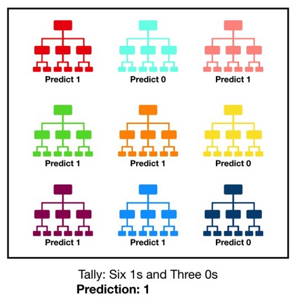
\includegraphics{./pic/chapter-4-2_pic_14.png}
\caption{chapter-4-2\_pic\_14.png}
\end{figure}

    The reason that the random forest model works is that a large number of
relatively uncorrelated models (trees) operating as a committee will
outperform any of the individual constituent models. The low correlation
between models is the key. Just like how investments with low
correlations (like stocks and bonds) come together to form a portfolio
that is greater than the sum of its parts, uncorrelated models can
produce ensemble predictions that are more accurate than any of the
individual predictions. The reason for this wonderful effect is that the
trees protect each other from their individual errors (as long as they
don't constantly all err in the same direction). While some trees may be
wrong, many other trees will be right, so as a group the trees are able
to move in the correct direction.

    \hypertarget{references}{%
\subsection{References}\label{references}}

    \begin{tcolorbox}[breakable, size=fbox, boxrule=1pt, pad at break*=1mm,colback=cellbackground, colframe=cellborder]
\prompt{In}{incolor}{ }{\boxspacing}
\begin{Verbatim}[commandchars=\\\{\}]

\end{Verbatim}
\end{tcolorbox}


    % Add a bibliography block to the postdoc
    
    
    
\end{document}
